\begin{apendicesenv}

\partapendices

\chapter{Grafos}

\section{Um Pouco mais de História}

Graças à resolução dada por Euler, mais tarde muitos outros problemas importantes, para o desenvolvimento da Matemática Aplicada, foram possíveis de serem modelados. Um desses modelos são as relações de amizade, de hierarquia, de trabalho. Netto \cite{Netto:2012}, aponta grafos como um auxílio para o estudo de problemas envolvendo inter-relacionamento de elementos (em química orgânica, eletricidade, organização, transporte, psicossociologia). Na verdade, grafos modelam diversas situações e muitas delas não quantificáveis.

Conforme Ore \cite{Ore:1963}, o matemático irlandês William Hamilton, em 1859, inventou um jogo chamado ``\textit{The Icosian Game}'', com um peculiar enigma envolvendo um dodecaedro, em que cada um dos 20 vértices foram nomeados com nomes de cidades importantes. O objetivo do jogo era, utilizando as 30 arestas do dodecaedro, passar por cada uma das cidades apenas uma vez, começando e terminando na mesma cidade. Um exemplo do grafo pode ser visualizado na figura \ref{grafo_hamiltoniano}.

\begin{figure}[!h]
	\centering
	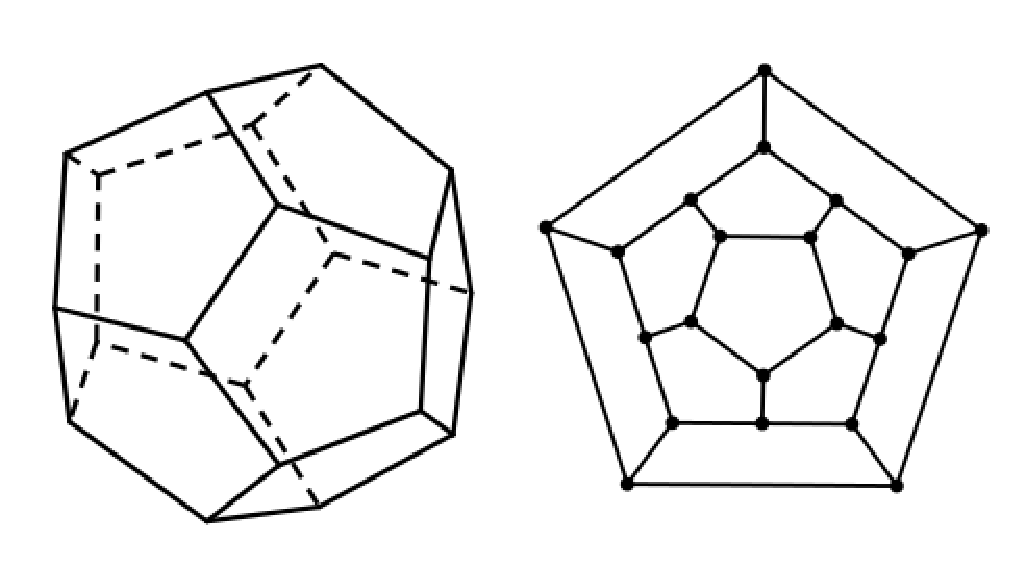
\includegraphics[scale=0.3]{figuras/referencial_teorico/grafo_hamiltoniano.eps}
	\caption[Grafo hamiltoniano]{Grafo hamiltoniano \cite{Ore:1963}}
	\label{grafo_hamiltoniano}
\end{figure}

Apesar da simples formulação, o problema admite muitos caminhos como resposta. No problema de Hamilton, temos uma diferença significativa em relação ao problema de Euler. Encontrar um caminho euleriano significa encontrar um caminho que passe por todas as arestas do grafo uma única vez, podendo ser aberto ou fechado. Nos caminhos hamiltonianos, cada vértice é visitado uma única vez. O problema fica mais complexo com tal condição \cite{Costa:2011}.

\section{Outras Definições}

Um grafo é finito se tanto o seu conjunto de vértices, quanto o seu conjunto de arestas são finitos. Um grafo sem vértices (e, portanto, sem arestas) é o grafo nulo. Qualquer grafo apenas com um vértice é referido como trivial. Todos os outros grafos são não-triviais \cite{Costa:2011}.

Um grafo é simples se não tem \textit{loops} ou arestas paralelas \cite{Diestel:1997}, como exemplificado na figura \ref{grafo_simples}.

\begin{figure}[!h]
	\centering
	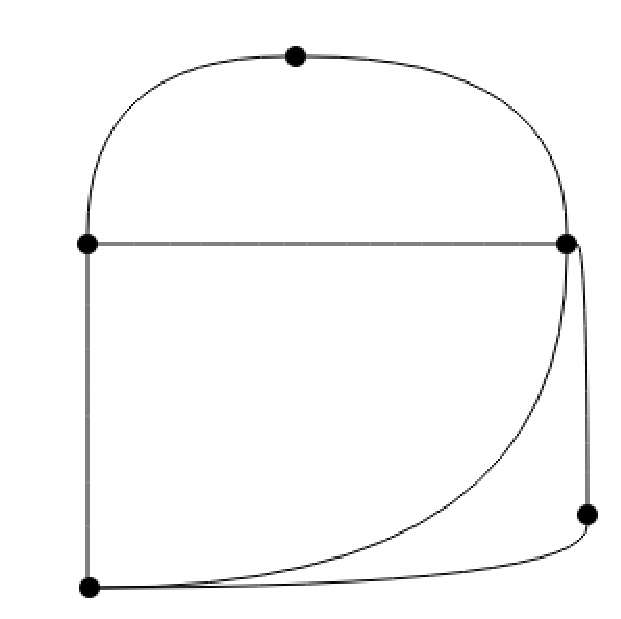
\includegraphics[scale=0.2]{figuras/referencial_teorico/grafo_simples.eps}
	\caption[Exemplo de grafo simples]{Exemplo de grafo simples \cite{Costa:2011}}
	\label{grafo_simples}
\end{figure}

Certos tipos de grafos podem desempenhar papéis proeminentes na teoria dos grafos. Um grafo conexo é um grafo simples no qual quaisquer dois vértices são ligados por um caminho. Um grafo é vazio quando não há dois vértices adjacentes (isto é, o conjunto de arestas é vazio). Um grafo é bipartido se o seu conjunto de vértices pode ser particionado em dois subconjuntos \textit{X} e \textit{Y} para que cada aresta tem um fim em \textit{X} e um fim em \textit{Y}; uma tal partição (\textit{X}, \textit{Y}) é chamada uma bipartição do grafo, e \textit{X} e \textit{Y} suas partes. Pode-se denotar um grafo bipartido \textit{G} com bipartição (\textit{X}, \textit{Y}) por \textit{G}[\textit{X}, \textit{Y}]. Se \textit{G}[\textit{X}, \textit{Y}] é simples e todos os vértices de \textit{X} estão associados a cada vértice em \textit{Y}, então \textit{G} é chamado de um grafo bipartido completo. Uma estrela é um grafo bipartido completo \textit{G}[\textit{X}, \textit{Y}] com |\textit{X}| = 1 ou |\textit{Y}| = 1 \cite{Diestel:1997}.  A figura \ref{tipos_grafos} ilustra estes tipos de grafos, sendo o grafo ``A'' é um grafo conexo, o grafo ``B'' é um grafo vazio e o grafo ``C'' é um grafo bipartido completo.

\begin{figure}[!h]
	\centering
	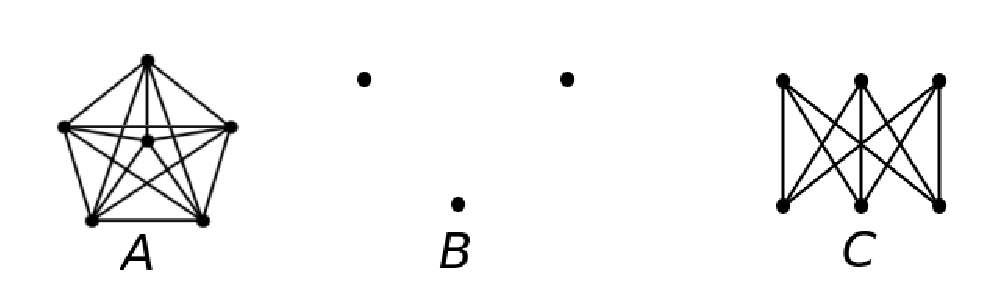
\includegraphics[scale=0.4]{figuras/referencial_teorico/tipos_grafos.eps}
	\caption[Tipos de grafos]{Tipos de grafos \cite{Diestel:1997}}
	\label{tipos_grafos}
\end{figure}

Um caminho é um grafo simples cujos vértices podem ser dispostos em uma sequência linear. De tal forma que dois vértices são adjacentes se forem consecutivos na sequência, e não adjacentes caso não forem consecutivos \cite{Bondy:2007}. Dessa forma, diz-se que um vértice é alcançável a partir de outro, se houver um caminho levando o primeiro vértice ao último \cite{Costa:2011}. A figura \ref{caminho} apresenta um caminho (arestas em vermelho) do vértice ``a'' até o vértice ``e''.

\begin{figure}[!h]
	\centering
	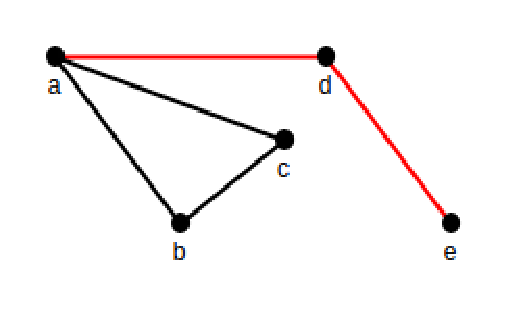
\includegraphics[scale=0.5]{figuras/referencial_teorico/caminho.eps}
	\caption[Caminho]{Caminho \cite{Costa:2011}}
	\label{caminho}
\end{figure}

Do mesmo modo, um ciclo é um grafo simples cujos vértices podem ser dispostos em uma sequência cíclica de tal maneira que dois vértices são adjacentes se forem consecutivos na sequência. O comprimento de um caminho ou de um ciclo é o número de suas arestas \cite{Costa:2011}. É possível observar na figura \ref{ciclos} alguns exemplos de grafos com ciclo.

\begin{figure}[!h]
	\centering
	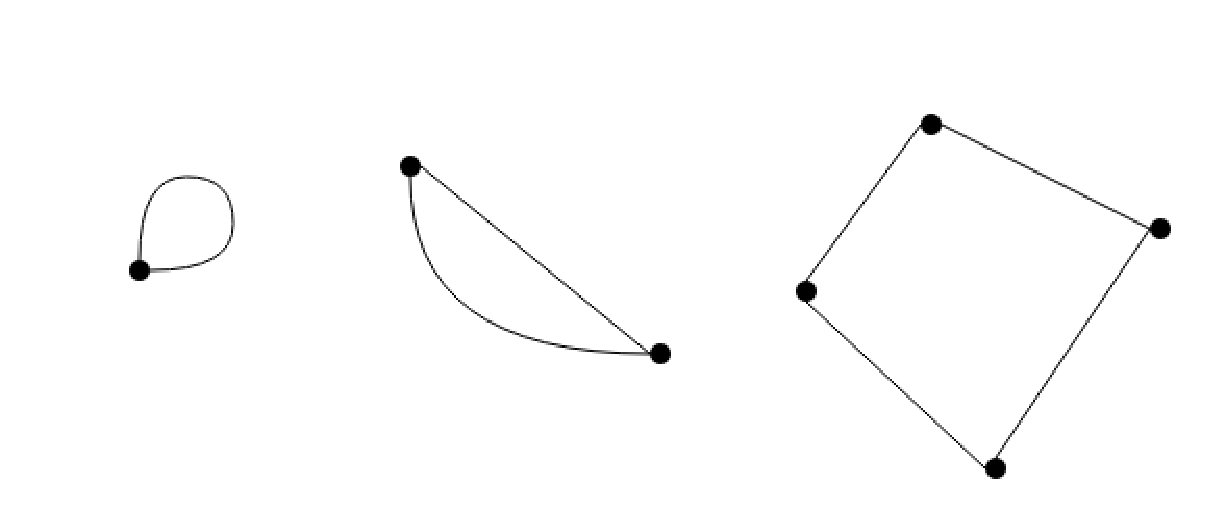
\includegraphics[scale=0.3]{figuras/referencial_teorico/ciclos.eps}
	\caption[Exemplo de grafos com ciclos]{Exemplo de grafos com ciclos \cite{Costa:2011}}
	\label{ciclos}
\end{figure}

Um grafo é conectado se, para cada partição de seus vértices definido em dois conjuntos \textit{X} e \textit{Y} não vazios, existe uma aresta com uma extremidade em \textit{X} e uma extremidade em \textit{Y}; caso contrário, o grafo é desconectado. Em outras palavras, um grafo é desconectado se o conjunto de vértices pode ser particionado em dois subconjuntos não vazios \textit{X} e \textit{Y} e que nenhuma aresta tem uma extremidade em \textit{X} e a outra extremidade em \textit{Y}. É instrutivo comparar esta definição com a de um grafo bipartido. Os exemplos de grafos conectados e desconectados são apresentados na figura \ref{desconectados}, onde o grafo ``X'' e o grafo ``Y'' são dois grafos distintos conectados. Porém se fossem trados como um único grafo, este seria um grafo desconectado \cite{Bondy:2007}.

\begin{figure}[!h]
	\centering
	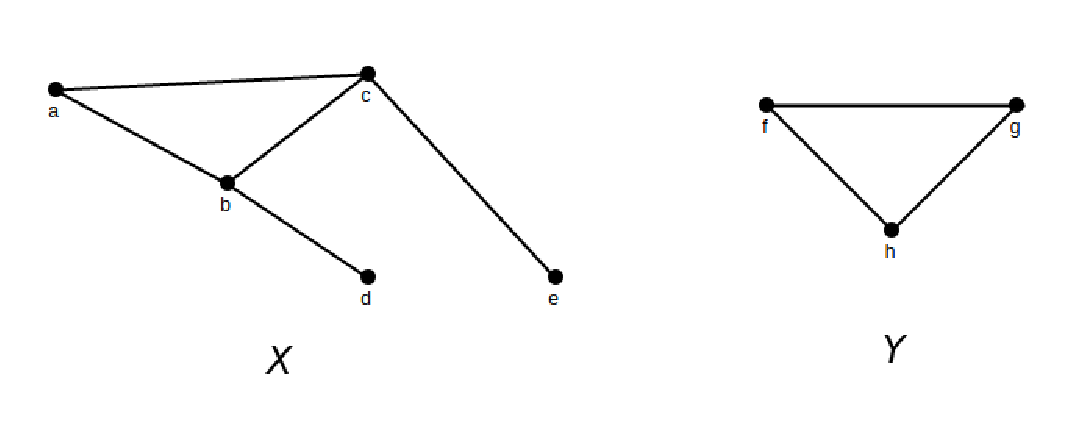
\includegraphics[scale=0.45]{figuras/referencial_teorico/desconectados.eps}
	\caption[Exemplo de grafos conectados e desconectados]{Exemplo de grafos conectados e desconectados \cite{Bondy:2007}}
	\label{desconectados}
\end{figure}

O grau de um vértice \textit{v} em um grafo \textit{G}, designado por \textit{d$_G$}(\textit{v}), é o número de arestas de \textit{G} que incidem em \textit{v}; para cada \textit{loop} é contado duas arestas. Em particular, se \textit{G} é um grafo simples, \textit{d$_G$}(\textit{v}) é o número de vizinhos de \textit{v} em \textit{G}. Um vértice de grau zero é chamado um vértice isolado. Denominamos por $\delta$(\textit{G}) e $\Delta$(\textit{G}) mínimo e máximo graus dos vértices de \textit{G}, e por \textit{d}(\textit{G}), o seu grau médio, $\frac{1}{n}\sum_{\textit{v}\in\textit{V}} \textit{d}(\textit{v})$ \cite{Diestel:1997}.

\chapter{Algoritmos}

\section{Complexidade de algoritmos}
\label{sec:complexidade_algoritmos}

Quando existem vários algoritmos que podem solucionar um problema, qual se deve escolher? Uma opção pode ser os algoritmos que possuem um fácil entendimento e depuração, porém dependendo do tipo de aplicação em que o algoritmo irá rodar, utilizar algoritmos que fazem um uso eficiente dos recursos do computador é essencial.

Para determinar qual algoritmo é mais eficiente que outro em determinado quesito, deve-se utilizar o cálculo de suas complexidades (custo). Este custo pode ser referente ao tempo de sua execução ou ao seu consumo de memória \cite{Albuquerque:2004}.

Para o cálculo de complexidade, pode-se medir o número de passos de execução em um modelo matemático denominado maquina de Turing, ou medir o número de segundos gastos em um computador específico. A medida de complexidade é o crescimento assintótico dessa contagem de operações \cite{Junior:2014}.

A objetivo de se fazer a análise de complexidade de um algoritmo é obter estimativas de tempos de execução do algoritmo \cite{Junior:2014}.

\subsection{Big O}

Uma das preocupações com a eficiência é com problemas que envolvem um grande número de elementos. Se existir uma tabela com apenas dez elementos, mesmo o algoritmo considerado menos eficiente resolvem o problema, no entanto, à medida que o número de elementos aumenta, o esforço necessário começa a fazer diferença de algoritmo para algoritmo. A notação \textit{Big O} faz uma estimativa de uma função de como o algoritmo se comporta com um número de elementos fixo ou tendendo ao infinito \cite{Junior:2014}. Pode-se observar na Figura \ref{grafico_complexidade} as principais funções que são utilizadas nesta notação.

Por exemplo, é mais importante saber que o número de operações executadas num algoritmo dobra se dobrarmos o valor de n, do que saber que para n igual a 100 são executadas 300 operações \cite{Junior:2014}.

\begin{figure}[!h]
	\centering
	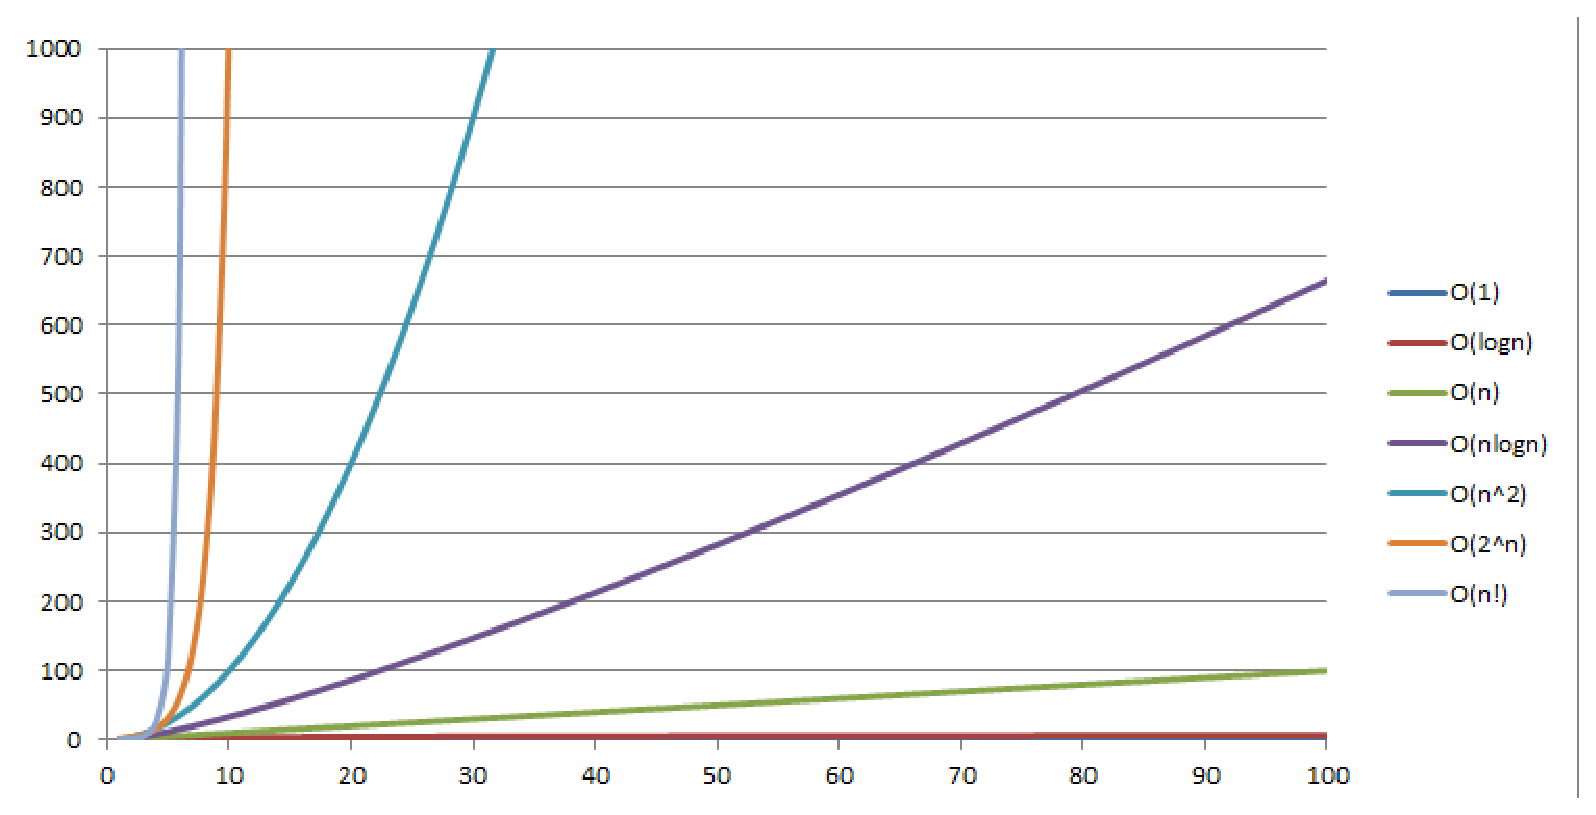
\includegraphics[scale=0.5]{figuras/apendices/grafico_complexidade.eps}
	\caption[Complexidade Big O]{Complexidade Big O}
	\label{grafico_complexidade}
\end{figure}

Os resultados expressos em notação \textit{Big O} devem ser interpretados com cuidado, pois indicam apenas que o tempo de execução do programa é proporcional a um determinado valor ou que nunca supera determinado valor. Na realidade o tempo de execução pode ser inferior ao valor indicado e pode ser que o pior caso nunca ocorra \cite{Junior:2014}.

\section{Busca em Grafos}

A busca em grafos refere-se ao método de explorar o grafo, ou seja, obter um método sistemático para percorrer seus vértices e arestas. Para isto, há dois principais algoritmos, busca em profundidade (\textit{DFS - Depth First Search}) e busca em largura (\textit{BFS - Breadth First Search}). Em ambos os casos parte-se de um vértice qualquer.

\subsection{DFS}
\label{subsec:dfs}

A ideia por trás do \textit{DFS} é alcançar ``mais fundo'' no grafo quanto possível. A ordem em que os vértices são visitados depende da ordem em que os vizinhos de cada vértice aparecem na lista de adjacência \cite{Cormen:2001}. A seguir é exemplificado um fluxo do funcionamento do DFS.

Considere as Figuras a seguir para a exemplificação do DFS.

\begin{figure}[!h]
	\centering
	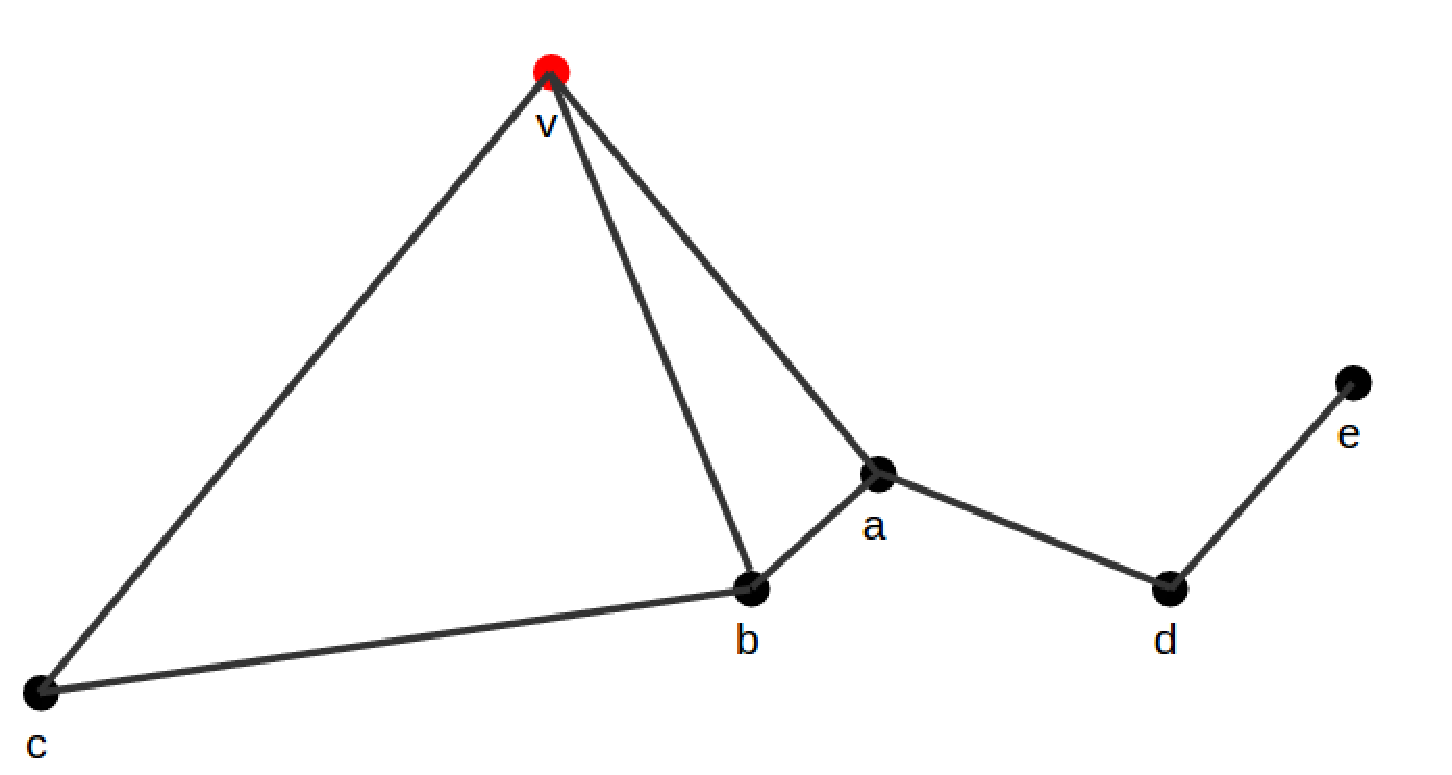
\includegraphics[scale=0.25]{figuras/referencial_teorico/dfs/dfs1.eps}
	\caption[Exemplo DFS etapa 1]{Exemplo DFS etapa 1 \cite{Cormen:2001}}
	\label{dfs1}
\end{figure}

A busca irá partir do vértice arbitrário \textit{v}, chamado de vértice raiz. A partir do vértice raiz é possível percorrer três arestas: (\textit{v}, \textit{a}), (\textit{v}, \textit{b}) e (\textit{v}, \textit{c}). A aresta a ser seguida será (\textit{v}, \textit{a}).

\newpage

\begin{figure}[!h]
	\centering
	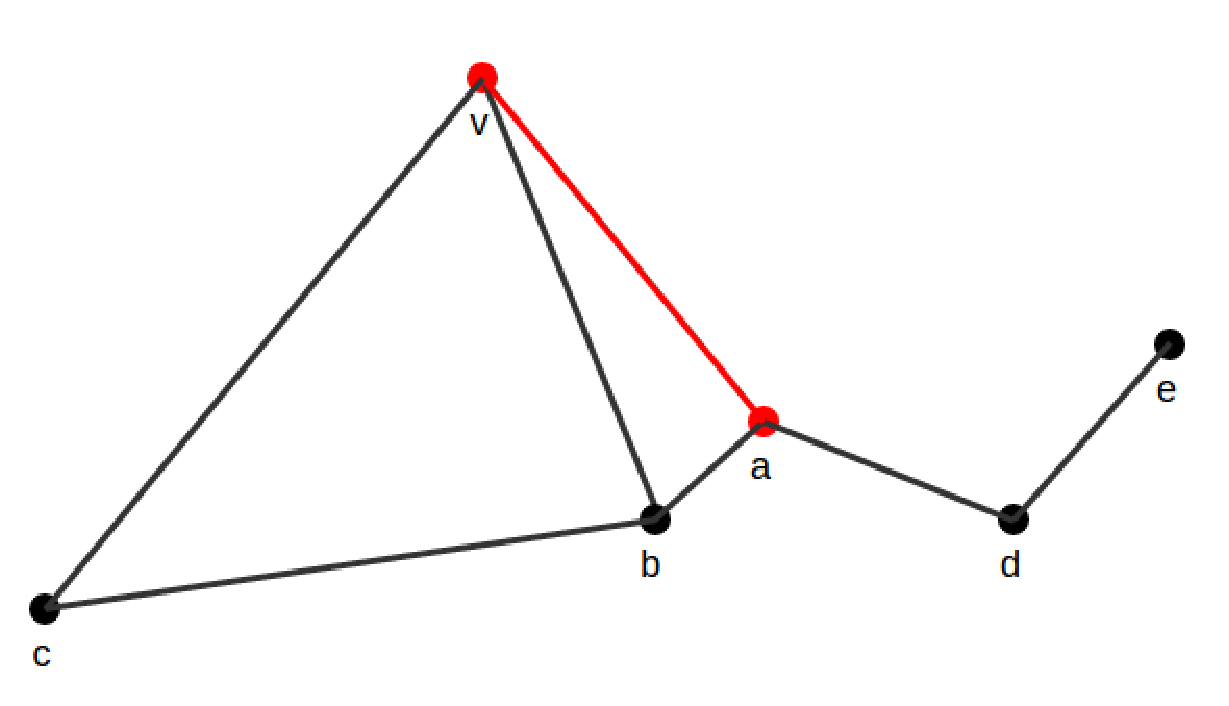
\includegraphics[scale=0.25]{figuras/referencial_teorico/dfs/dfs2.eps}
	\caption[Exemplo DFS etapa 2]{Exemplo DFS etapa 2 \cite{Cormen:2001}}
	\label{dfs2}
\end{figure}

O vértice \textit{a} possui três arestas, que são: (\textit{a}, \textit{v}), (\textit{a}, \textit{b}) e (\textit{a}, \textit{d}). Como o vértice \textit{v} já foi visitado, a aresta a ser seguida será (\textit{a}, \textit{b}).

\begin{figure}[!h]
	\centering
	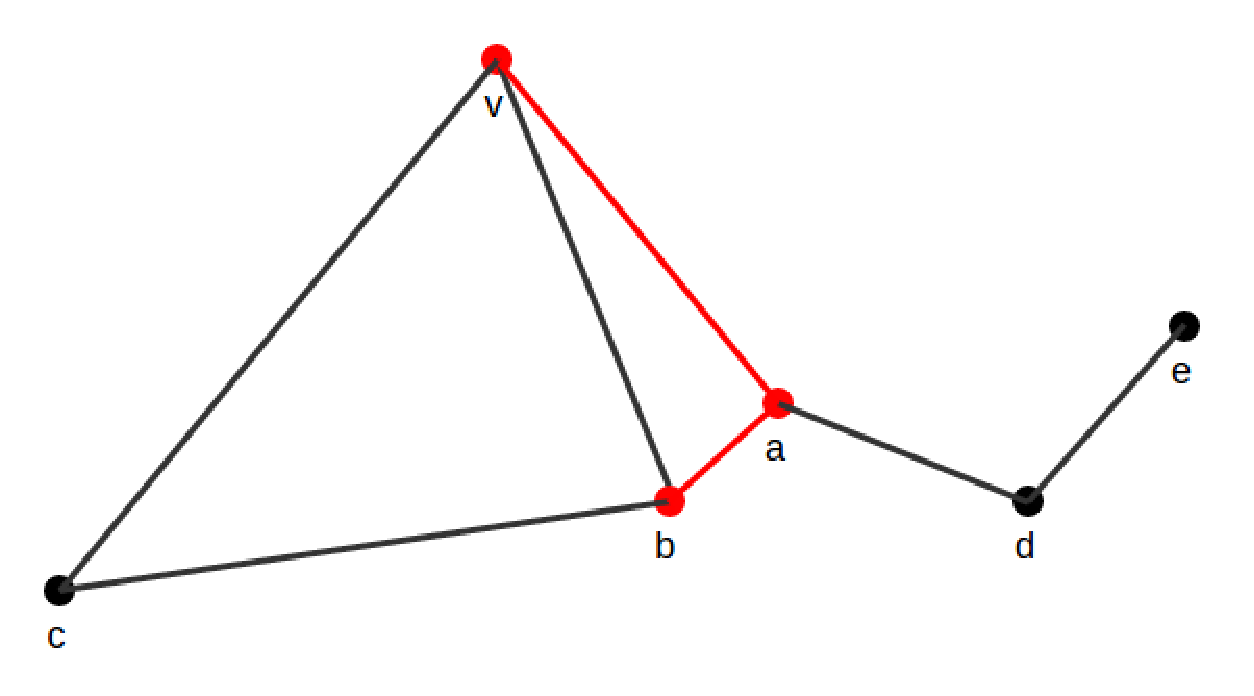
\includegraphics[scale=0.25]{figuras/referencial_teorico/dfs/dfs3.eps}
	\caption[Exemplo DFS etapa 3]{Exemplo DFS etapa 3 \cite{Cormen:2001}}
	\label{dfs3}
\end{figure}

A partir de \textit{b}, é possível escolher as seguintes arestas: (\textit{b}, \textit{v}), (\textit{b}, \textit{a}) e (\textit{b}, \textit{c}). Porém como os vértices \textit{v} e \textit{a} já foram visitados, a opção restante será a aresta (\textit{b}, \textit{c}).

\begin{figure}[!h]
	\centering
	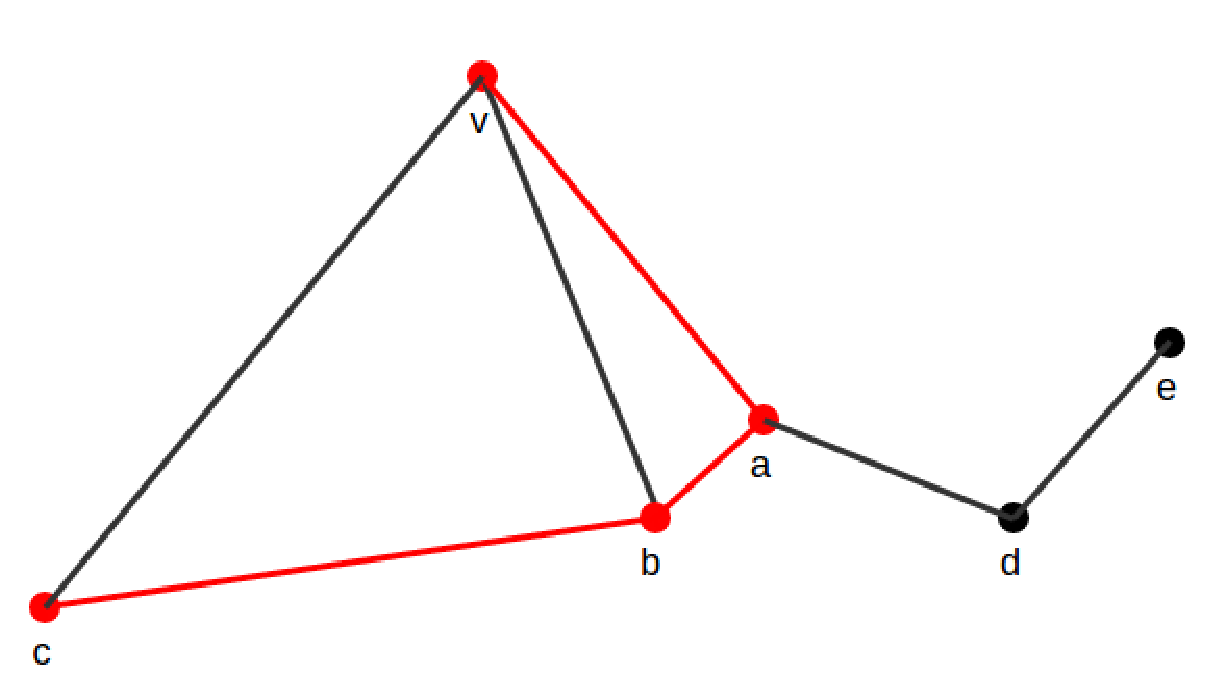
\includegraphics[scale=0.25]{figuras/referencial_teorico/dfs/dfs4.eps}
	\caption[Exemplo DFS etapa 4]{Exemplo DFS etapa 4 \cite{Cormen:2001}}
	\label{dfs4}
\end{figure}

Ao alcançar \textit{c}, há duas possibilidades: (\textit{c}, \textit{v}) e (\textit{c}, \textit{b}). Porém ambos os vértices \textit{v} e \textit{b} já são conhecidos. Neste caso não há para onde se aprofundar. Entretanto, ainda existem vértices não descobertos. Nesse caso, deve-se voltar até o vértice \textit{b}, verificando se há alguma aresta que leva a um vértice ainda não visitado. Caso ocorra tal situação, deve-se voltar novamente pelo caminho percorrido, chegando ao vértice \textit{a}. Em \textit{a}, a aresta (\textit{a}, \textit{d}) leva a um vértice ainda não descoberto, portanto, esse caminho deve ser tomado.

\begin{figure}[!h]
	\centering
	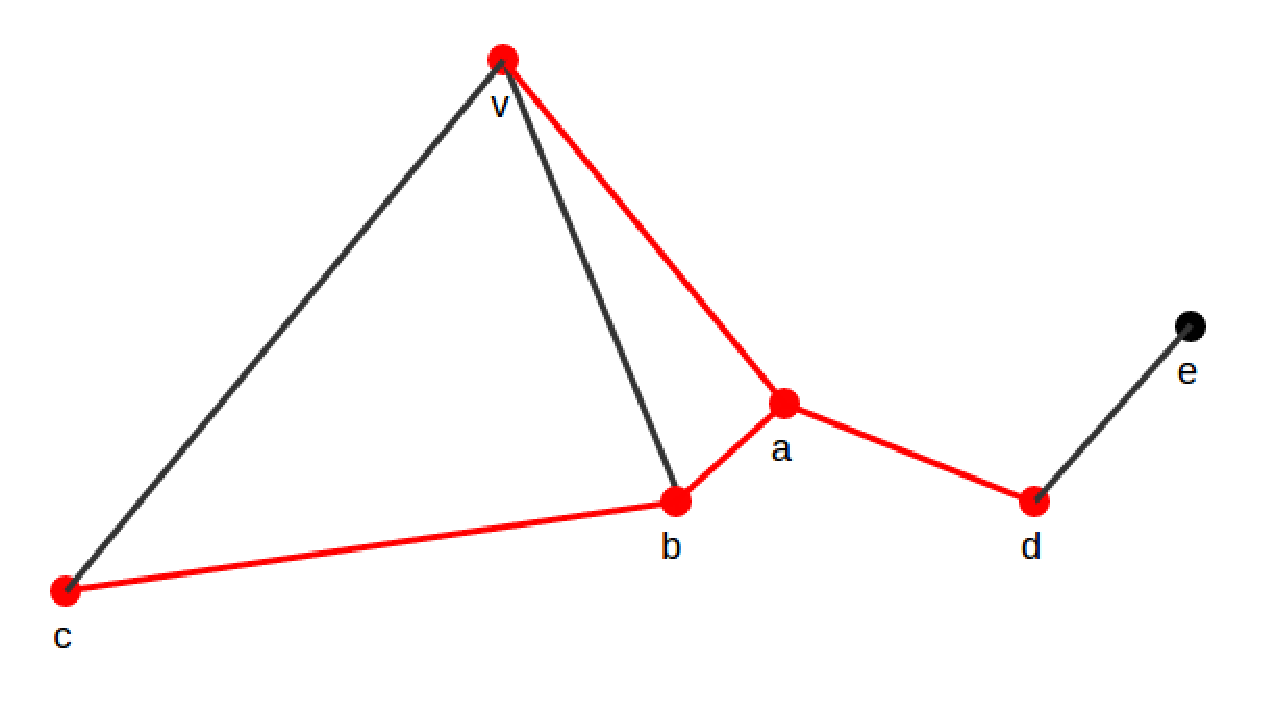
\includegraphics[scale=0.25]{figuras/referencial_teorico/dfs/dfs5.eps}
	\caption[Exemplo DFS etapa 5]{Exemplo DFS etapa 5 \cite{Cormen:2001}}
	\label{dfs5}
\end{figure}

Em \textit{d}, há dois caminhos a seguir: (\textit{d}, \textit{a}) e (\textit{d}, \textit{e}). Porém a única aresta que leva a um vértice não visitado é (\textit{d}, \textit{e}). Esta deverá ser seguida.

\begin{figure}[!h]
	\centering
	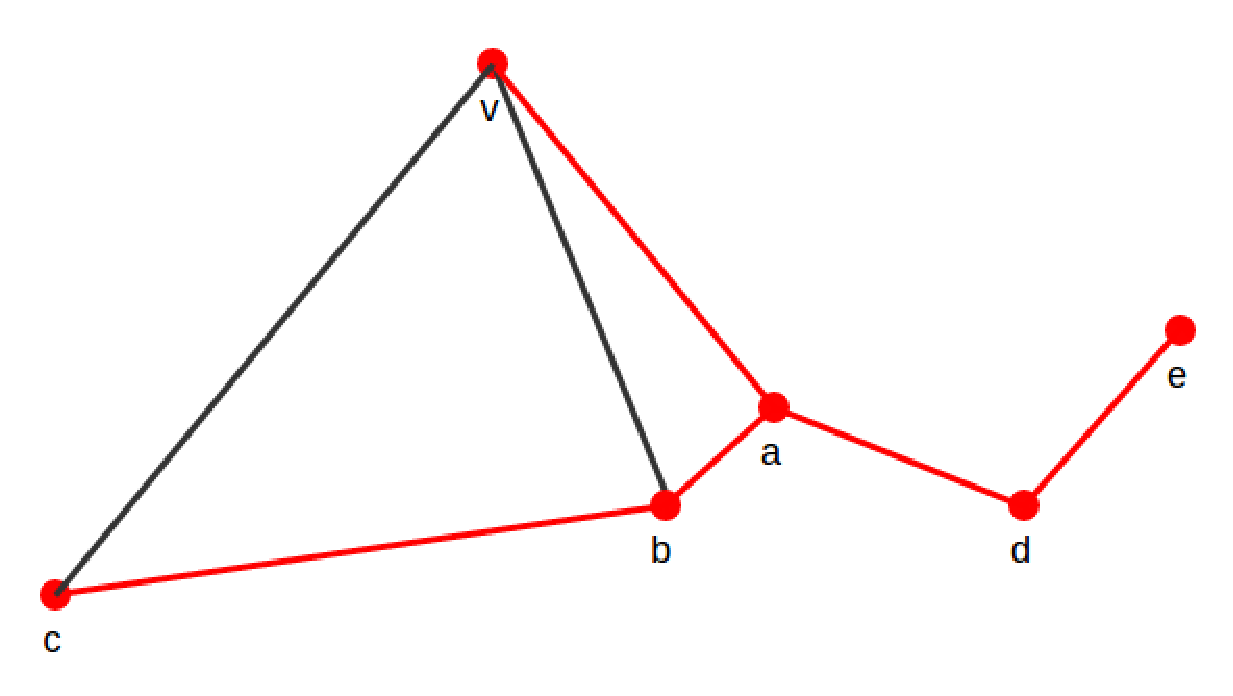
\includegraphics[scale=0.25]{figuras/referencial_teorico/dfs/dfs6.eps}
	\caption[Exemplo DFS etapa 6]{Exemplo DFS etapa 6 \cite{Cormen:2001}}
	\label{dfs6}
\end{figure}

Ao alcançar o vértice \textit{e}, não existem vértices não visitados, mesmo na volta no caminho. Portanto, o percurso realizado pelo \textit{DFS} pode ser observado na figura \ref{dfs_percurso}, o qual é uma árvore.

\begin{figure}[!h]
	\centering
	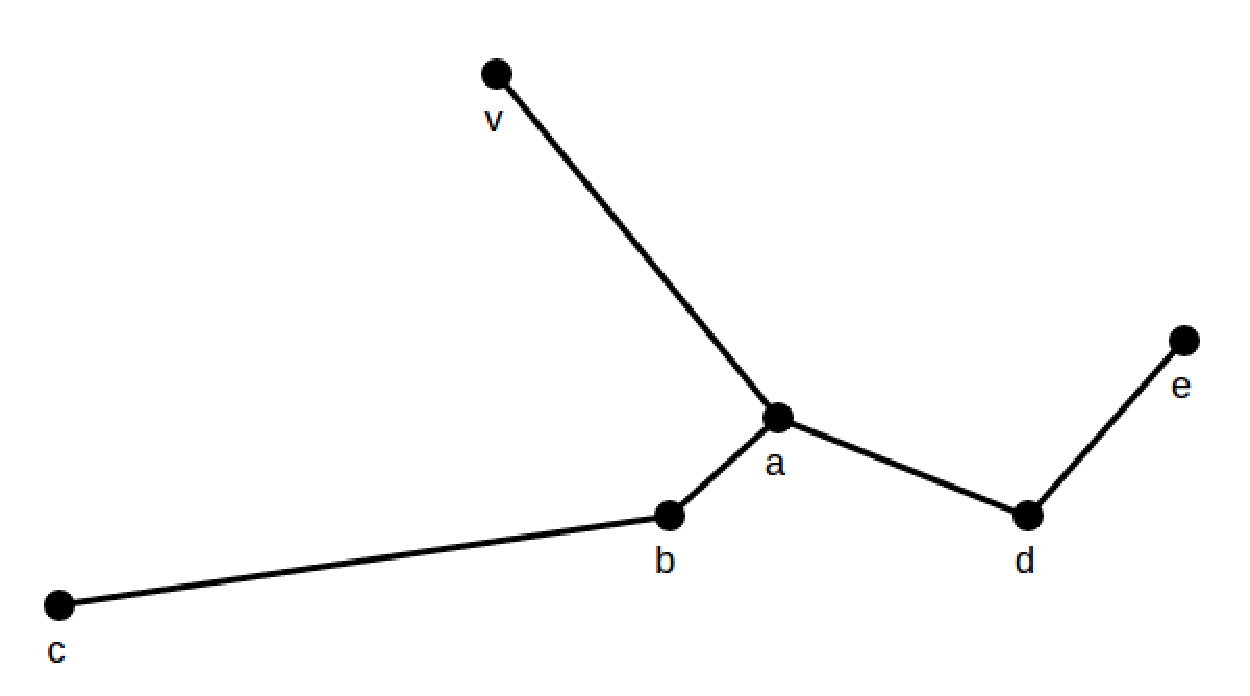
\includegraphics[scale=0.25]{figuras/referencial_teorico/dfs/dfs_percurso.eps}
	\caption[Percurso do DFS]{Percurso do DFS \cite{Cormen:2001}}
	\label{dfs_percurso}
\end{figure}

\subsection{BFS}
\label{subsec:bfs}

O \textit{DFS}, a partir de um vértice \textit{v}, tenta visitar algum vizinho deste, em seguida, um vizinho deste vizinho, e assim por diante. O \textit{BFS}, a partir de um vértice \textit{v}, visita todos os vizinhos de \textit{v}. Quando visitado todos os vizinhos de um vértice, os vizinhos destes vizinhos serão visitados \cite{Brassard:1988}.

A Figura \ref{bfs} exemplifica o algoritmo da busca \textit{BFS}, onde as letras significam o estado da busca e a ordem de cada estado. Os vértices marcados como vermelho representam que estes já foram visitados; os vértices marcados como azul representam que estes vértices serão os próximos a serem visitados.

\begin{figure}[!h]
	\centering
	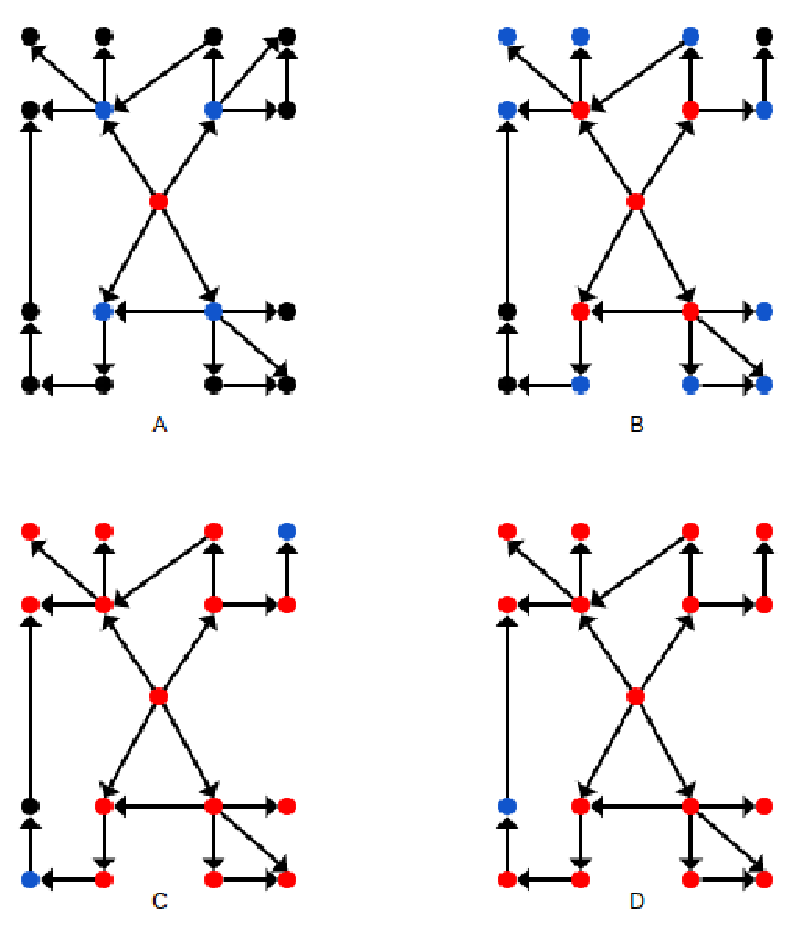
\includegraphics[scale=0.55]{figuras/referencial_teorico/bfs.eps}
	\caption[Percurso do BFS]{Percurso do BFS \cite{Brassard:1988}}
	\label{bfs}
\end{figure}

\chapter{Reutilização de Software}
\label{chapter:reutilizacao_software}

\section{Serviços}
\label{sec:servicos}

De uma maneira geral, serviços são atividades providas e realizadas por uma máquina ou um humano. No desenvolvimento de software, serviços são considerados um bloco de construção reutilizável que oferece uma funcionalidade particular. A noção de reusabilidade apresentada lembra a reutilização antes comentada no conceito de componentes. De fato, essas duas abordagens estão próximas, pois representam uma ideia de desenvolvimento comum, onde blocos de software são construídos para serem usados por atores diferentes e em outros locais \cite{Stojanovic:Dahanayake:2005}.

Com o advento dos serviços, surgiu um novo termo, a ``Orientação a serviços''. Essa ocorre quando alguns processos são modelados e construídos como unidades bem definidas e formam serviços. Esses são encapsulados em componentes de software para serem usados por outras aplicações, conferindo a ideia de um sistema provedor (o sistema que provê o serviço) e um sistema consumidor (que consome os serviços prestados) \cite{Victorino:Brascher:2009}.

Se todas as aplicações usassem a mesma interface de programação e o mesmo protocolo de interoperabilidade, todo trabalho de software seria mais simples. Essa é a premissa que trouxe o desenvolvimento orientado a serviços para o mundo da tecnologia da informação. Quando se desenvolve dessa forma, os serviços tornam-se a base para a criação de novas estratégias de solução \cite{Newcomer:Lomow:2004}.

Apesar das abordagens de orientação a serviços e orientação a componentes serem bem similares, no livro \cite{Stojanovic:Dahanayake:2005}, são apresentadas algumas diferenças entre as mesmas, que são:

\begin{itemize}
	\item o tempo de integração. Na orientação baseada em componentes, a integração com a aplicação desenvolvida ocorre no momento da construção; enquanto, na orientação a serviços, a integração pode ocorrer antes ou durante a execução, pois apenas as descrições dos serviços estão disponíveis no momento da execução;
	\item nos serviços, o foco é a descoberta, existindo uma ênfase mais forte na separação entre a descrição do serviço e a implementação. Nos componentes, é a composição, onde as partes são integradas diretamente na aplicação;
	\item serviços são mais voltados para tarefas dinâmicas, ao contrário dos componentes que são mais voltados para pontos estáticos. Porém, esse comportamento dinânmico pode ser feito também em componentes, e;
	\item a orientação a componentes atribui maior responsabilidade para o ambiente e a execução da própria aplicação. Os serviços não são necessariamente dessa forma, pois podem estar presentes em outras máquinas e outros servidores externos.
\end{itemize}

A seguir serão apresentadas duas formas conhecidas e já consolidadas de implementações de serviços, os \textit{Web Services} e os \textit{Serviços RESTful}.

\subsection{Web Services}

Os serviços são informatizados por tecnologias interoperáveis, que são capazes de se comunicar entre si, e isso independe da plataforma e da linguagem de programação utilizadas. Dentre essas tecnologias, os ``\textit{Web Services}'' (serviços web) se destacam. Esses serviços fornecem um modo padronizado de integrar aplicativos web, e assim, organizações podem se comunicar sem que uma tenha conhecimento abrangente dos sistemas da outra \cite{Victorino:Brascher:2009}.

Um ``\textit{Web Service}'' é uma noção abstrata que deve ser implementada por um agente concreto, sendo esse agente um pedaço de software que envia e recebe mensagens. O serviço é o recurso caracterizado pela funcionalidade abstrata que é servida.

O XML hoje é amplamente utilizado quase como o protocolo HTTP, e faz parte da solução para aplicação de ``\textit{Web Services}''. Normalmente, usado para realizar a formatação dos dados \cite{Alonso:Casati:Kuno:Machiraju:2010}.

Simplificando, os ``\textit{Web Services}'' possuem três características e tecnologias principais que são usadas para desenvolvê-los: o XML, que é a especificação sobre a qual estes são construídos; o WSDL, que provê as interfaces fundamentais que serão usadas, e SOAP, que é responsável pela comunicação com outros serviços. Pode-se dizer que um ``\textit{Web Service}'' deve fornecer interfaces de uso simples e se comunicar facilmente com outros serviços \cite{Newcomer:Lomow:2004}.

\subsection{Serviços RESTFul}

REST é um estilo arquitetural para sistemas hipermídia distribuídos, reunindo um grupo de critérios que serão incorporados ao projeto de aplicações distribuídas. Os Serviços RESTful são serviços web que seguem os critérios REST \cite{Filho:2009}.

O uso de serviços RESTFul permitiu grande impulso no desenvolvimento de aplicações distribuídas baseadas em padrões WEB tradicionais. Esses serviços são leves, práticos e fáceis de serem integrados em várias aplicações \cite{Rosenberg:Curbera:Duftler:Khalaf:2008}.

Os serviços da web estão a cada dia buscando soluções mais simples e mais leves para compor suas funcionalidades. Os serviços RESTFul introduzem um novo tipo de abstração que busca oferecer as funcionalidades já existentes dos serviços da \textit{web} comuns. Porém, de uma forma mais leve e simples \cite{Pautasso:2009}.

De acordo com \cite{Filho:2009}, os serviços RESTFul possuem cinco conceitos importantes, que são descritos a seguir:

\begin{itemize}
	\item \textbf{recurso:} é uma abstração ou conceito relevante para o domínio tratado. Os recursos podem ser concretos ou abstratos, e têm-se maior flexibilidade para definição dos mesmos. Um serviço pode ter mais de um recurso sem afetar a sua qualidade;
	\item \textbf{representação:} é a representação de um recurso, apresentando informações sobre o mesmo. Dependendo do serviço e do nível de abstração, são mostradas mais ou menos informações dos recursos. A representação é uma serialização do recurso em uma linguagem específica, as mais usadas são: XML, XHTML e JSON. Um serviço pode mostrar mais de um tipo de serialização de seus recursos, basta que as requisições informem qual o formato desejado que o serviço irá apresentar os dados na serialização correta;
	\item \textbf{identificador uniforme:} cada recurso deve ter ao menos um identificador para localização do mesmo. Se não existe um identificador uniforme, não se pode considerar que um objeto é um recurso. Pode-se ter ilimitados identificadores para um mesmo recurso.
	\item \textbf{interface unificada:} A interface unificada diz respeito a todos os serviços utilizarem o mesmo protocolo, no caso, o HTTP. Dessa forma, um cliente que conheça esse protocolo pode facilmente utilizar os métodos que são proporcionados por ele para fazer requisições nos serviços disponíveis, e;
	\item \textbf{escopo de execução:} neste caso, o serviço RESTFul também se utiliza do protocolo HTTP, porém, diz respeito aos parâmetros que devem ser enviados junto da requisição para que o serviço possa tratar o recurso corretamente. Pode ser, por exemplo, a identificação de um objeto em um conjunto de recursos.
\end{itemize}

\section{Padrão Abstract Factory}
\label{sec:padrao_abstract_factory}

A seguir, têm-se uma breve descrição do padrão ``\textit{Abstract Factory}'', como foi definido em \cite{Gamma:1995}.

Esse padrão fornece uma estrutura para criação de famílias de objetos relacionados sem a necessidade de definir suas classes concretas. A figura \ref{abstract_factory} apresenta o modelo do ``\textit{Abstract Factory}''.

\begin{figure}[!h]
	\centering
	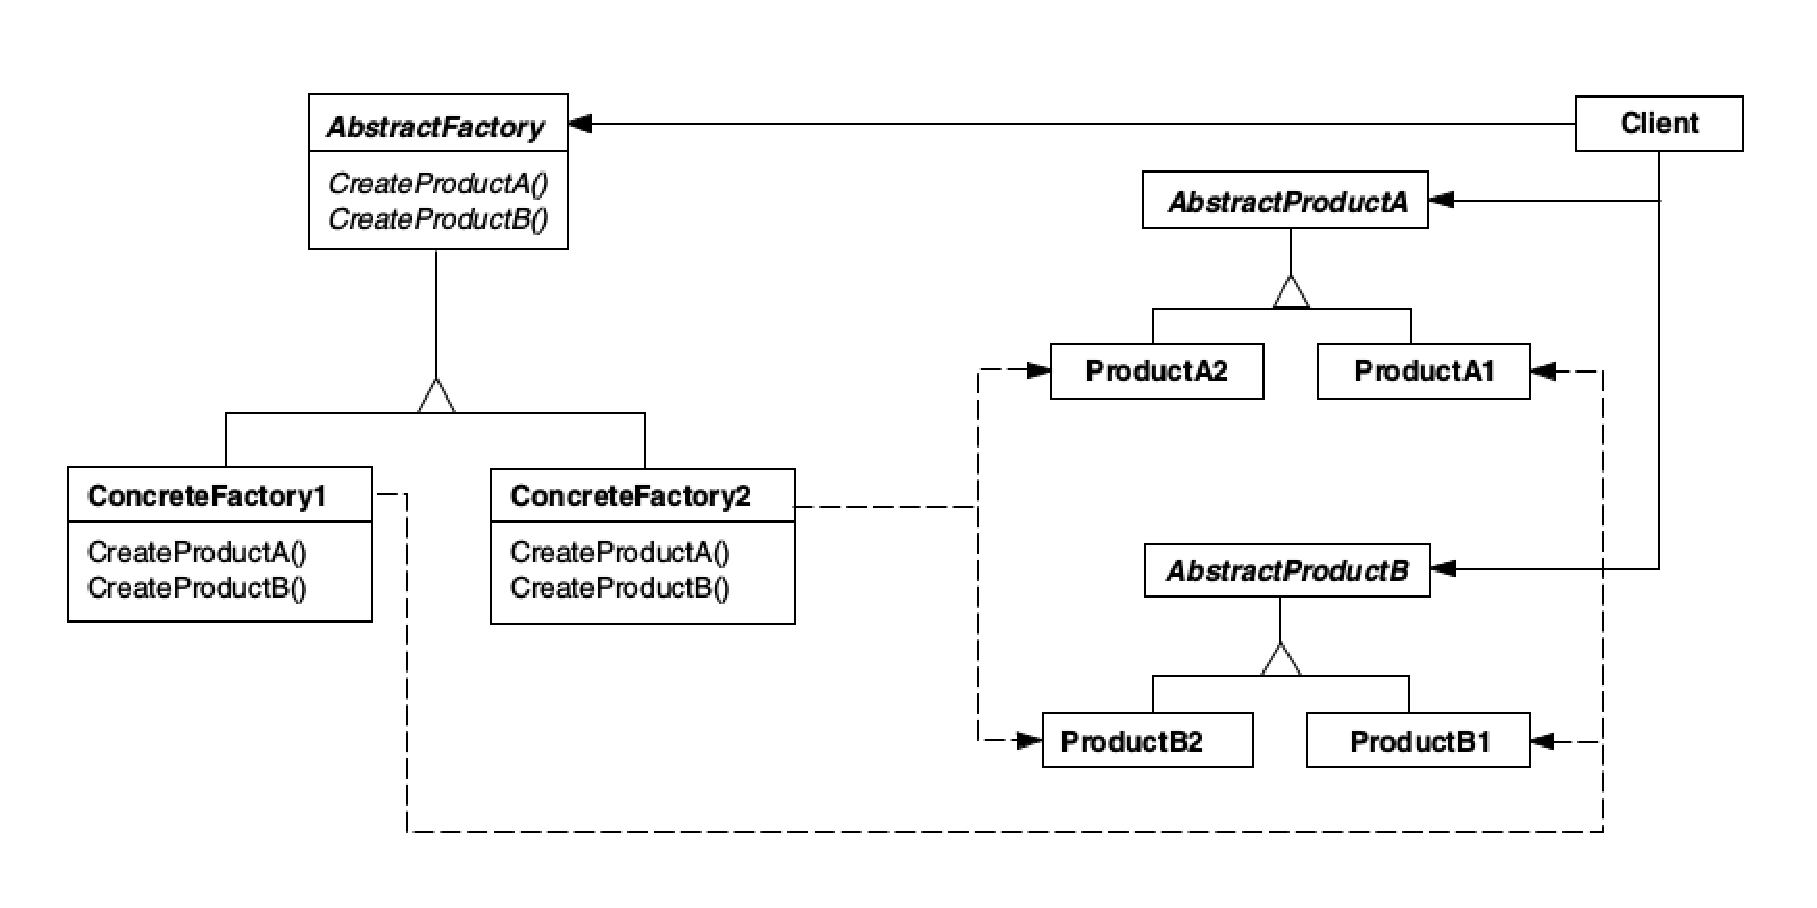
\includegraphics[scale=0.5]{figuras/apendices/abstract_factory.eps}
	\caption[Modelo genérico do Abstract Factory]{Modelo genérico do Abstract Factory \cite{Gamma:1995}}
	\label{abstract_factory}
\end{figure}

O modelo da figura apresenta cinco tipos de classes. ``\textit{Abstract Factory}'', ``\textit{Concrete Factory}'', ``\textit{Abstract Product}'', ``\textit{Product}'' e ``\textit{Client}''.

\begin{itemize}
	\item \textbf{\textit{Abstract Factory:}} Faz declarações de interfaces para criação de quaisquer produtos;
	\item \textbf{\textit{Concrete Factory:}} Essas classes já estão focadas no tipo de produtos que vão criar e implementam os métodos abstratos para essa criação;
	\item \textbf{\textit{Abstract Product:}} Classes abstratas que declaram interfaces para um determinado tipo de produto que deverá ser criado;
	\item \textbf{\textit{Product:}} Classes que representam o próprio produto que deverá ser criado, são as classes que são chamadas pelos métodos de criação presentes nas ``\textit{Concrete Factory}'';
	\item \textbf{\textit{Client:}} É a classe que representa quem irá fazer as chamadas aos métodos de criação. Não é necessário que conheça de fato as classes concretas de produto, pois apenas faz uso das interfaces declaradas em ``\textit{Abstract Factory}'' e ``\textit{Abstract Product}''; a primeira para criar os produtos, e a segunda para usá-los.
\end{itemize}

Este padrão oferece algumas vantagens e desvantagens que são apresentadas a seguir:

\begin{itemize}
	\item \textbf{Isolamento de classes concretas:} O cliente pode trabalhar com as criações dos produtos sem necessariamente conhecer as classes concretas que existem por traz, pois este trabalha apenas com as interfaces abstratas providas.
	\item \textbf{Fácil troca de famílias de produtos:} Basta trocar qual é a classe concreta que deverá ser usada que todo o comportamento dos produtos irá se alterar de acordo com essa classe. Isso pode ser feito facilmente no momento de instanciação da fábrica.
	\item \textbf{Harmonia entre produtos:} Como o padrão permite aos clientes trabalharem apenas com uma família por vez, fica fácil alcançar harmonia, pois todos os produtos da família estão de alguma forma relacionados.
	\item \textbf{Suporte a novos tipos de produtos é difícil:} Como a interface do ``\textit{Abstract Factory}'', no início, cria uma quantidade fixa de produtos para serem implementados, alterar isso fica difícil, pois é necessário mexer na classe principal e criar as subclasses concernentes.
\end{itemize}

\section{Padrão Factory Method}
\label{sec:padrao_factory_method}

Um outro padrão de criação bem parecido com o \nameref{sec:padrao_abstract_factory}, porém, diferentemente do anterior que cria famílias de objetos, o \textit{Factory Method} é responsável por criar um único objeto \cite{Gamma:1995}. A figura \ref{factory_method} apresenta o modelo de classes desse padrão:

\newpage
\begin{figure}[!h]
	\centering
	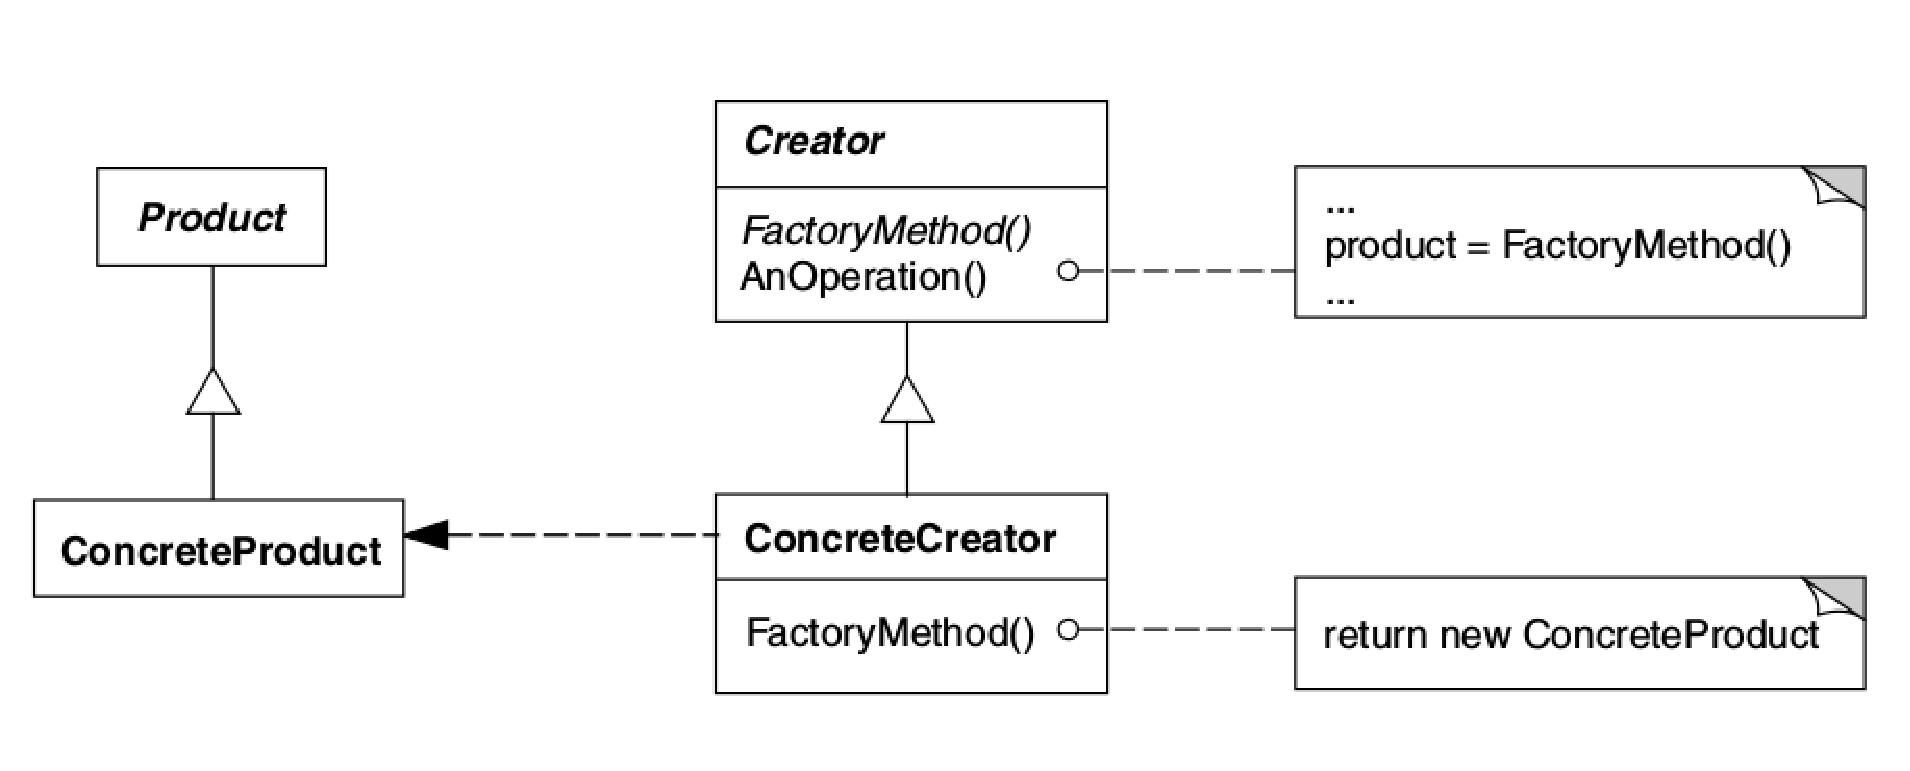
\includegraphics[scale=0.5]{figuras/apendices/factory_method.eps}
	\caption[Modelo genérico do Factory Method]{Modelo genérico do Factory Method \cite{Gamma:1995}}
	\label{factory_method}
\end{figure}

Com esse padrão fica fácil e prático fazer a alteração de uma sub-classe concreta, uma vez que, a aplicação passa a trabalhar com a interface de ``\textit{Product}'', o código pode trabalhar com quaisquer classes ``\textit{ConcrectProduct}'' definidas pelo usuário.

As classes mostradas no modelo são descritas a seguir:

\begin{itemize}
	\item \textbf{\textit{Product}}: Interface de objetos que o método de fábrica irá criar;
	\item \textbf{\textit{ConcretProduct}}: Implementação da interface ``\textit{Product}'';
	\item \textbf{\textit{Creator}}: Interface com método para criação de um ``\textit{Product}'';
	\item \textbf{\textit{ConcrectCreator}}: Implementação da interface ``\textit{Creator}'', reimplementa o método para criação de um ``\textit{ConcrectProduct}''.
\end{itemize}

\section{Padrão Strategy}
\label{sec:padrao_strategy}

O padrão ``\textit{Strategy}'' foi desenvolvido para auxiliar desenvolvedores a trabalhar com famílias de algoritmos que podem variar independentemente dos clientes que os usam \cite{Gamma:1995}. Com esse padrão é possível mudar facilmente o comportamento de um dado algoritmo apenas trocando a classe que é usada na implementação do mesmo. A seguir é apresentado o modelo de classes desse padrão na figura \ref{strategy}.

\newpage
\begin{figure}[!h]
	\centering
	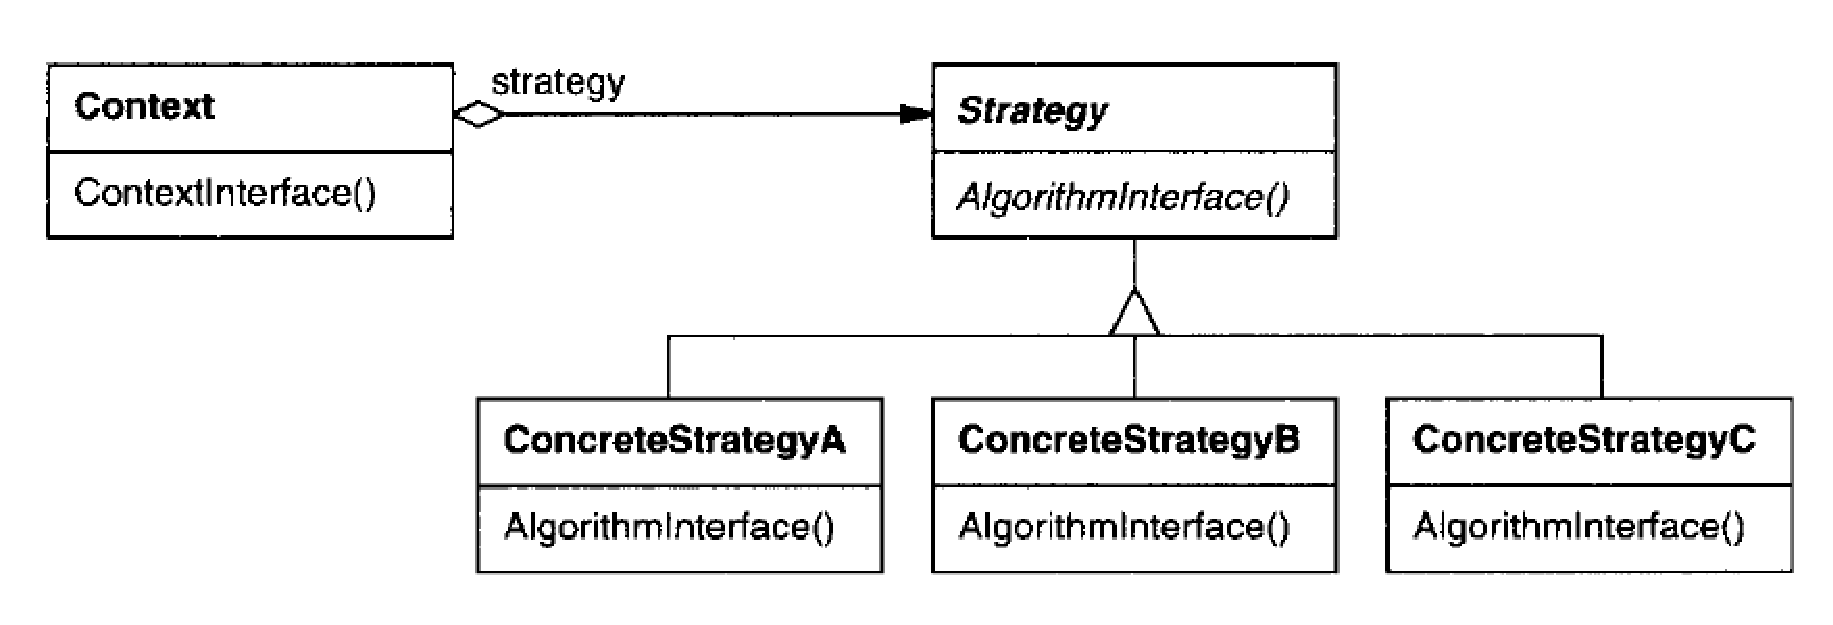
\includegraphics[scale=0.5]{figuras/apendices/strategy.eps}
	\caption[Modelo genérico do Strategy]{Modelo genérico do Strategy \cite{Gamma:1995}}
	\label{strategy}
\end{figure}

As classes do modelo são descritas a seguir.

\begin{itemize}
	\item \textbf{\textit{Strategy}}: Interface comum para todos os algoritmos que serão suportados.
	\item \textbf{\textit{ConcretStrategy}}: Implementação da interface ``\textit{Strategy}'' definindo cada método com um comportamento esperado para um determinado cliente;
	\item \textbf{\textit{Context}}: Essa classe faz uso da interface ``\textit{Strategy}'' chamando cada um de seus métodos através de um objeto ``\textit{ConcretStrategy}'' que é definido, sendo assim,  o comportamento esperado será retornado de acordo com o ``\textit{ConcretStrategy}'' que é passado.
\end{itemize}

\chapter{Metodologia}
\label{apend_chap:metodologia}

Metodologias específicas colaboram para estabelecer diretrizes e boas práticas na condução do trabalho, conferindo padronização, noções de pesquisa científica, dentre outras contribuições \cite{Wohlin:2000}.

A metodologia pode ser entendida como um conjunto de etapas a serem realizadas na condução do processo investigativo em um determinado contexto. É a metodologia que define os passos que serão seguidos para realização das pesquisas, escolha do tema, planejamento da investigação, desenvolvimento, coleta e análise dos dados, análise dos resultados e conclusões a respeito das lições aprendidas \cite{Moresi:2003}.

Pesquisar significa identificar uma dúvida que necessite ser esclarecida, construir e executar o processo que apresente a solução desta, quando não há teorias que a expliquem ou quando as teorias que existem não estão aptas para fazê-lo \cite{Koche:1997}. A seguir, serão apresentadas as formas de se classificar uma pesquisa.

\section{Classificação da pesquisa}

\begin{itemize}
	\item Do ponto de vista da natureza da pesquisa, esta pode ser:
		\begin{itemize}
			\item \textbf{Pesquisa Básica:} Possui o objetivo de gerar novos conhecimentos para a ciência. Neste tipo de pesquisa não é obrigatório que o conhecimento gere um uso prático \cite{Silva:Tafner:2007}.
			\item \textbf{Pesquisa Aplicada:} Visa gerar uma maior compreensão para assuntos práticos dirigidos à solução de problemas específicos \cite{Silva:Tafner:2007}.
		\end{itemize}

	\item Do ponto de vista da forma de abordagem do problema,tem-se:
		\begin{itemize}
			\item \textbf{Pesquisa Quantitativa:} O estudo quantitativo considera que tudo pode ser quantificável, ou seja, que os números podem ser classificados, gerando informações ao analisá-los, através da análise estatística \cite{Travassos:2002}.
			\item \textbf{Pesquisa Qualitativa:} O estudo qualitativo está relacionado à pesquisa sobre os objetos, quando os resultados são apresentados em termos naturais, usando conjuntos nebulosos, porcentagens de satisfação, dentre outras formas de classificar algo subjetivo \cite{Travassos:2002}.
		\end{itemize}

	\item Do ponto de vista de seus objetivos, tem-se:
		\begin{itemize}
			\item \textbf{Pesquisa Exploratória:} Esta pesquisa tem como objetivo proporcionar maior familiaridade com o problema, possibilitando o aprimoramento de ideias ou a descoberta de intuições \cite{Gil:2010}.
			\item \textbf{Pesquisa Descritiva:} Seu principal objetivo é a descrição das características de determinada população ou fenômeno ou, então, o estabelecimento de relações entre variáveis \cite{Gil:2010}.
			\item \textbf{Pesquisa Explicativa:} Tem como preocupação central identificar os fatores que determinam ou que contribuem para a ocorrência dos fenômenos. Esse é o tipo de pesquisa que mais aprofunda o conhecimento da realidade, porque explica a razão, o porquê das coisas \cite{Gil:2010}.
		\end{itemize}

	\item Do ponto de vista dos procedimentos técnicos, pode ser:
		\begin{itemize}
			\item \textbf{Pesquisa Bibliográfica:} Visa encontrar as fontes primárias e secundárias e os materiais científicos e tecnológicos necessários para a realização do trabalho científico ou técnico-científico. Muitos estudos fazem uso do levantamento bibliográfico ou são desenvolvidas exclusivamente por fontes bibliográficas. Sua principal vantagem é possibilitar ao investigador a cobertura de uma gama de acontecimentos muito ampla \cite{Silva:Tafner:2007}.

			\item \textbf{Pesquisa Documental:} Assemelha-se à pesquisa bibliográfica. Porém, esta é realizada a partir de materiais que não receberam tratamento analítico. Por exemplo, reportagens de jornal, cartas, contratos, diários, filmes, fotografias e gravações. A pesquisa documental pode ser realizada ainda através de documentos de segunda mão, que de alguma forma já foram analisados. Por exemplo, relatórios de empresas e tabelas estatísticas \cite{Gil:2010}.

			\item \textbf{Levantamento:} É uma investigação realizada em retrospecto, que em seguida, mediante análise quantitativa, chega às conclusões correspondentes aos dados coletados. O levantamento feito com informações de todos os integrantes do universo da pesquisa origina um censo. \cite{Mafra:Travassos:2006}.
			
			\item \textbf{Estudo de Caso:} São estudos conduzidos com o propósito de se investigar uma entidade ou um fenômeno dentro de um espaço de tempo específico. Estes são usados principalmente para a monitoração de atributos presentes em projetos, atividades ou atribuições. Durante a sua condução, dados são coletados e analisados estatisticamente de forma a permitir a avaliação de um determinado atributo ou do relacionamento entre diferentes atributos. \cite{Mafra:Travassos:2006}
			
			\item \textbf{Pesquisa-Ação:} É realizada em conjunto com uma ação ou com a resolução de um problema coletivo, visando definir o campo de investigação, as expectativas dos interessados e o tipo de auxílio que estes poderão exercer ao longo do processo de pesquisa. Esta pesquisa implica no contato direto com o campo de estudo, envolvendo o reconhecimento visual do local, consulta a documentos diversos e a discussão com os envolvidos na pesquisa. A abordagem dos problemas dos grupos investigados na pesquisa-ação é mais qualitativa do que quantitativa \cite{Silva:Tafner:2007}.
			
			\item \textbf{Pesquisa Participante:} A intenção é obter um maior conhecimento sobre o grupo. O grupo investigado tem ciência da finalidade, dos objetivos da pesquisa e da identidade do pesquisador. A pesquisa participante permite a observação das ações no próprio momento em que ocorrem \cite{Silva:Tafner:2007}.
			
			\item \textbf{Pesquisa Experimental:} É conduzida quando deseja-se obter um maior controle da situação, ao se manipular as variáveis envolvidas no estudo de forma direta, sistemática e precisa. A pesquisa experimental necessita de previsão de relações entre as variáveis a serem estudadas, como também o seu controle. O objetivo é manipular uma ou mais variáveis e controlar todas as outras variáveis em um valor fixo. O efeito da manipulação das variáveis é então medido e, baseado nessa medição, análises estatísticas são conduzidas. A condução de experimentos reais é rara em Engenharia de Software, devido à dificuldade de se alocar os participantes do estudo a diferentes tratamentos de forma aleatória. Nessas situações, tais estudos denominam-se quasi-experimentos \cite{Mafra:Travassos:2006}.
			
			\item \textbf{Pesquisa Ex-Post-Facto:} Realizada quando o experimento se dá depois dos fatos. Neste caso, o pesquisador não tem controle sobre as variáveis. Esta pesquisa difere da pesquisa experimental pelo fato de o fenômeno ocorrer naturalmente sem que o pesquisador tenha controle sobre ele, ou seja, o pesquisador passa a ser um mero observador do acontecimento \cite{Silva:Tafner:2007}.
		\end{itemize}

\end{itemize}

\chapter{Prova de Conceito}
\label{chap:prova_conceito}

Foi desenvolvida uma pequena aplicação para implementação de alguns conceitos discutidos neste trabalho.

De modo geral, a aplicação desenvolvida implementa uma rede de usuários ligados entre si, formando um grafo. A solução contêm as classes \textit{User}, \textit{Edge} e \textit{Graph}. A classe \textit{Edge} é usada para fazer as ligações entre as entidades. A classe \textit{Graph} representa a própria rede com todos os usuários. A classe de \textit{User} pode ser vista como os vértices do grafo. Foram implementadas as funcionalidades de relacionamento descritas nas figuras \ref{segue} e \ref{amigo}, além de uma varredura dos usuários presentes no grafo pelos algoritmos de busca ~\nameref{subsec:bfs}, \textit{Breadth-First Search}, e ~\nameref{subsec:dfs}, \textit{Depth-First Search}.

A Figura \ref{modelo prova de conceito} apresenta o modelo das classes desenvolvidas na aplicação de prova de conceito e seus respectivos relacionamentos.

\begin{figure}[!h]
	\centering
	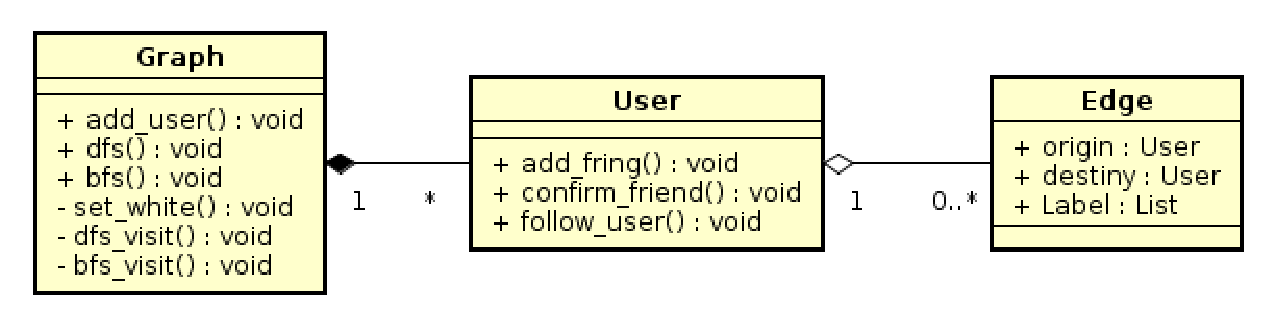
\includegraphics[scale=0.8]{figuras/proposta/classes_prova_conceito.eps}
	\caption{Classes da prova de conceito}
	\label{modelo prova de conceito}
\end{figure}

Fica exemplificado o relacionamento entre as classes \textit{Graph} e \textit{User} na forma de uma composição, que indica que um usuário não pode existir sem estar presente na rede. O relacionamento entre usuários, como pode ser visto na Figura \ref{modelo prova de conceito}, é feito através das arestas que possuem: (i) um atributo \textit{origin}, que representa de qual usuário parte o relacionamento e (ii) um atributo \textit{destiny}, que representa a qual usuário é indicado o relacionamento criado. Cada aresta possui ainda uma lista de \textit{labels} que representam os nomes dos relacionamentos entre os usuários.

Pode-se ver ainda na Figura \ref{modelo prova de conceito} a apresentação dos métodos construídos. A classe \textit{User} possui os métodos responsáveis por estabelecer os relacionamentos entre usuários, conforme apresentado nas figuras \ref{segue} e \ref{amigo}. O método \textit{``follow\_user''} é responsável por criar um relacionamento unidirecional, que representa seguir um usuário. O método \textit{``add\_friend''} é responsável por relacionamentos bidirecionais. Este último, por sua vez, necessita ainda ser complementado pelo método \textit{``confirm\_friend''}, pois, ao se invocar o método \textit{``add\_friend''} cria-se uma aresta que possui o \textit{label} amigo e pendente, o que indica que o relacionamento ainda não está completo. Ao se invocar o método \textit{``confirm\_friend''}, outra aresta é criada no outro sentido e o \textit{label} pendente é removido, completando-se assim, o relacionamento entre os dois usuários.

A classe \textit{Graph} possui o método \textit{``add\_user''}, que é chamado sempre na criação de um novo usuário, visando adicionar este a rede. O método \textit{``set\_white''} tem como objetivo definir a cor de todos os usuários no grafo para branco. Esse atributo é usado ao se trabalhar com os recursos de buscas no grafo. Colorir o nó com a cor branca significa que este ainda não foi visitado. O método \textit{``dfs''} implementa o algoritmo de busca ~\nameref{subsec:dfs} e faz uma varredura no grafo. O mesmo acontece para o método \textit{``bfs''} que implementa a varredura de acordo com o algoritmo ~\nameref{subsec:bfs}. Os métodos \textit{``dfs\_visit''} e \textit{``bfs\_visit''} são métodos auxiliares que visitam o nó corrente e definem o próximo nó que será visitado de acordo com as regras definidas nos algoritmos.

A abordagem de lista de adjacência foi utilizada na implementação do grafo. Como as arestas trabalhadas possuem outras informações além da representação das ligações entre os nós, essa abordagem ocupa menos espaço em memória. Isso ocorre pois não existe representação de arestas que não estejam presentes no grafo. Além da redução da memória gasta, o tempo gasto para listar todos os nós que fazem ligação a um outro nó é reduzido, quando se usa lista de adjacência, pois basta realizar a leitura da lista para se obter essas informações. Já na matriz de adjacência e incidência, é necessário realizar uma busca em uma linha da matriz para verificar todas as ligações que um nó possui. O código fonte dessa aplicação pode ser encontrado em \url{https://github.com/TCC-SocialNetwork/concept-test}.

\chapter{Suporte Tecnológico}
\label{chapter:Suporte_Tecnologico}

A fim de manter e disponibilizar o código e os artefatos gerados a partir deste trabalho, bem como o ambiente utilizado para a construção do \textit{framework}, serão apresentadas as principais ferramentas que foram utilizadas durante o seu desenvolvimento.

\section{Ferramentas de Desenvolvimento}

\subsection{Git}

Este trabalho utulizou o Git\footnote{\url{https://git-scm.com/}} (versão 1.9.1) como o sistema de controle de versão. O Git foi projetado basicamente para facilitar a vida de quem quer executar projetos em equipe de forma segura. Foi criado por Linus Torvalds, que precisava de um controle de versão rápido e que pudesse lidar com as atividades envolvidas no desenvolvimento do Kernel do Linux. Linus desejava um ferramenta livre; não encontrando, decidiu criar o Git. Esse suporte foi nomeado em referência ao próprio Linus, pois no inglês britânico, \textit{git} é uma gíria para ``cabeça-dura''.

Uma vantagem do Git é a possibilidade de controlar o projeto de forma descentralizada, ou seja, sem a exigência de um servidor mestre. A cada arquivo rastreado pelo Git, tem seu conteúdo verificado através do algoritmo de criptografia SHA-1\footnote{\url{http://www.training.com.br/lpmaia/pub_seg_cripto.htm}}.

O que faz o Git funcionar é sua habilidade de detectar mudanças em arquivos, não só que uma mudança ocorreu, mas também onde essa mudança ocorreu. Dessa forma, as alterações com problemas podem ser desfeitas, voltando para a versão estável.

\subsection{GitHub}

O GitHub\footnote{\url{https://github.com}}, lançado em 2008 e escrito em Ruby on Rails, provê um armazenamento em nuvem (\textit{Cloud}), onde se pode hospedar projetos que utilizam o Git como controle de versão. O GitHub possui funcionalidades de uma rede social como \textit{feeds}, \textit{followers}, wiki e gráficos para apresentar como os desenvolvedores trabalham em um repositório. Este lado social é interessante para descobrir novos projetos e receber ajuda em projetos particulares. É importante ressaltar que o repositório fornecido pelo GitHub é gratuito, e este repositório fica como de acesso público. Entretanto, existem planos comerciais nos quais o repositório pode se tornar privado.

A seguir é apresentada, na Figura \ref{github}, a tela de um repositório hospedado no GitHub.

\begin{figure}[!h]
	\centering
	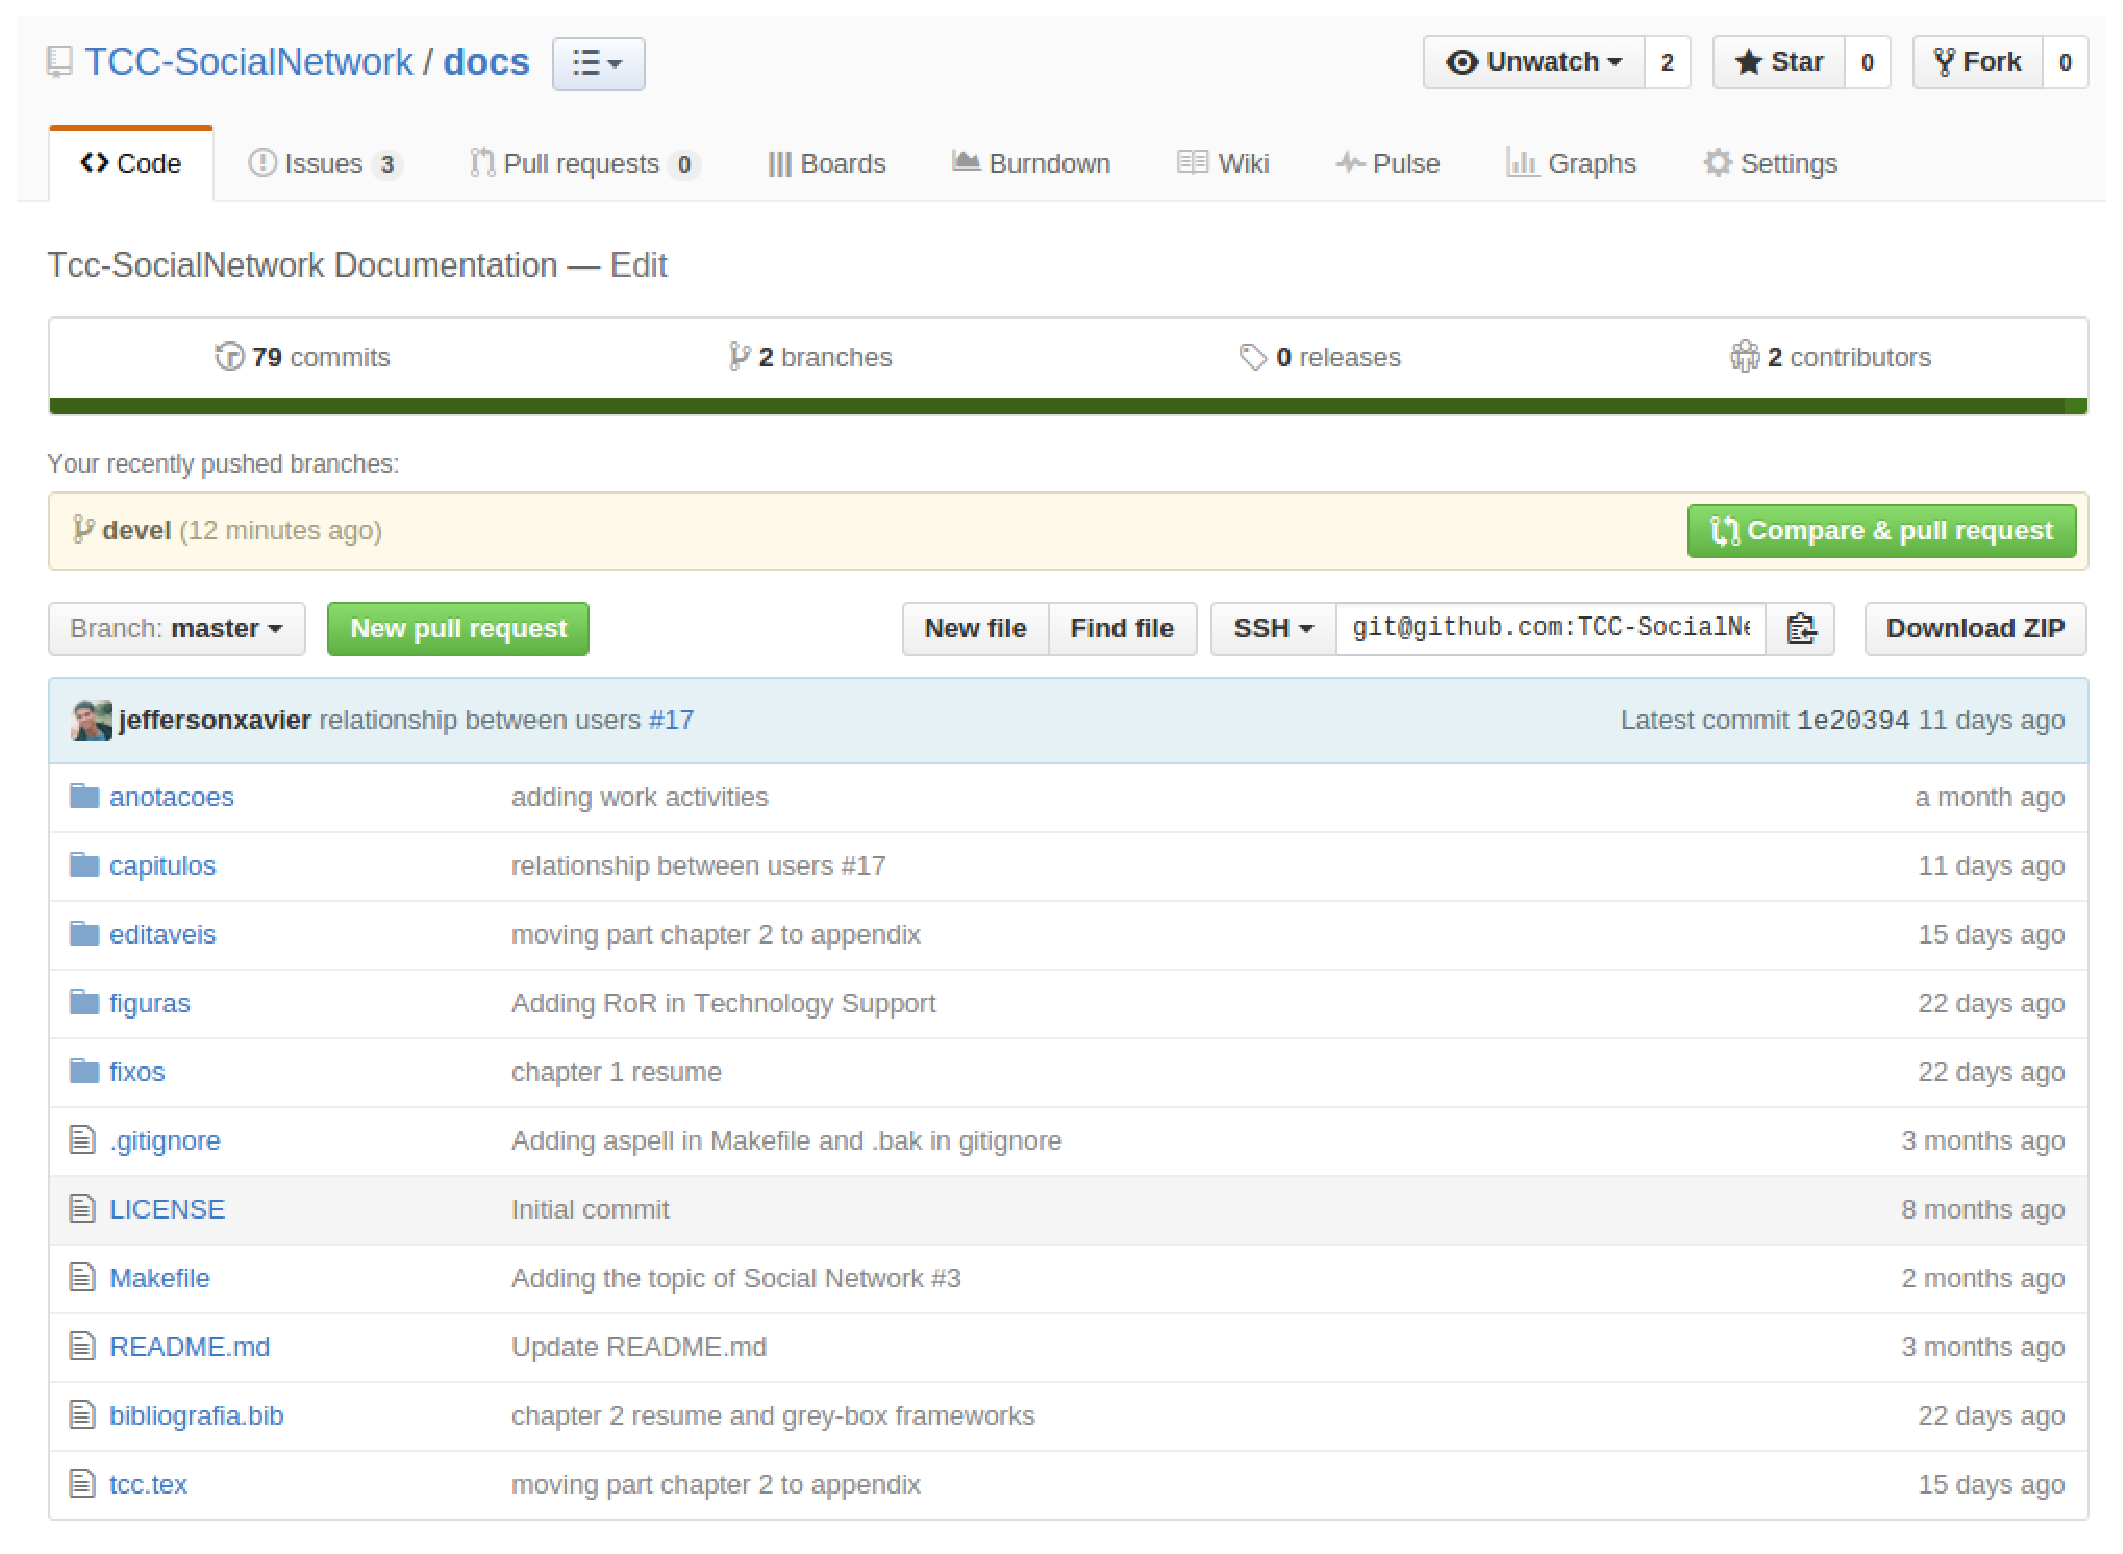
\includegraphics[scale=0.35]{figuras/ferramentas/github.eps}
	\caption{Repositório no GitHub}
	\label{github}
\end{figure}

\subsection{Waffle}

O Waffle\footnote{\url{https://waffle.io}} é um gerenciador de projetos gratuito conectado aos \textit{Pull Requests} e as \textit{Issues} do GitHub, que visa facilitar o trabalho das equipes de engenharia no que se refere ao acompanhamento das tarefas de uma forma visual, mostrando-as em um quadro com divisões para cada fase.

O Waffle escuta as ações em seu fluxo de trabalho para saber quando o trabalho é iniciado, quando está pronto para revisão, ou quando está finalizado e atualiza seu status automaticamente.

A Figura \ref{waffle} apresenta um exemplo de um \textit{board} do Waffle.

\newpage

\begin{figure}[!h]
	\centering
	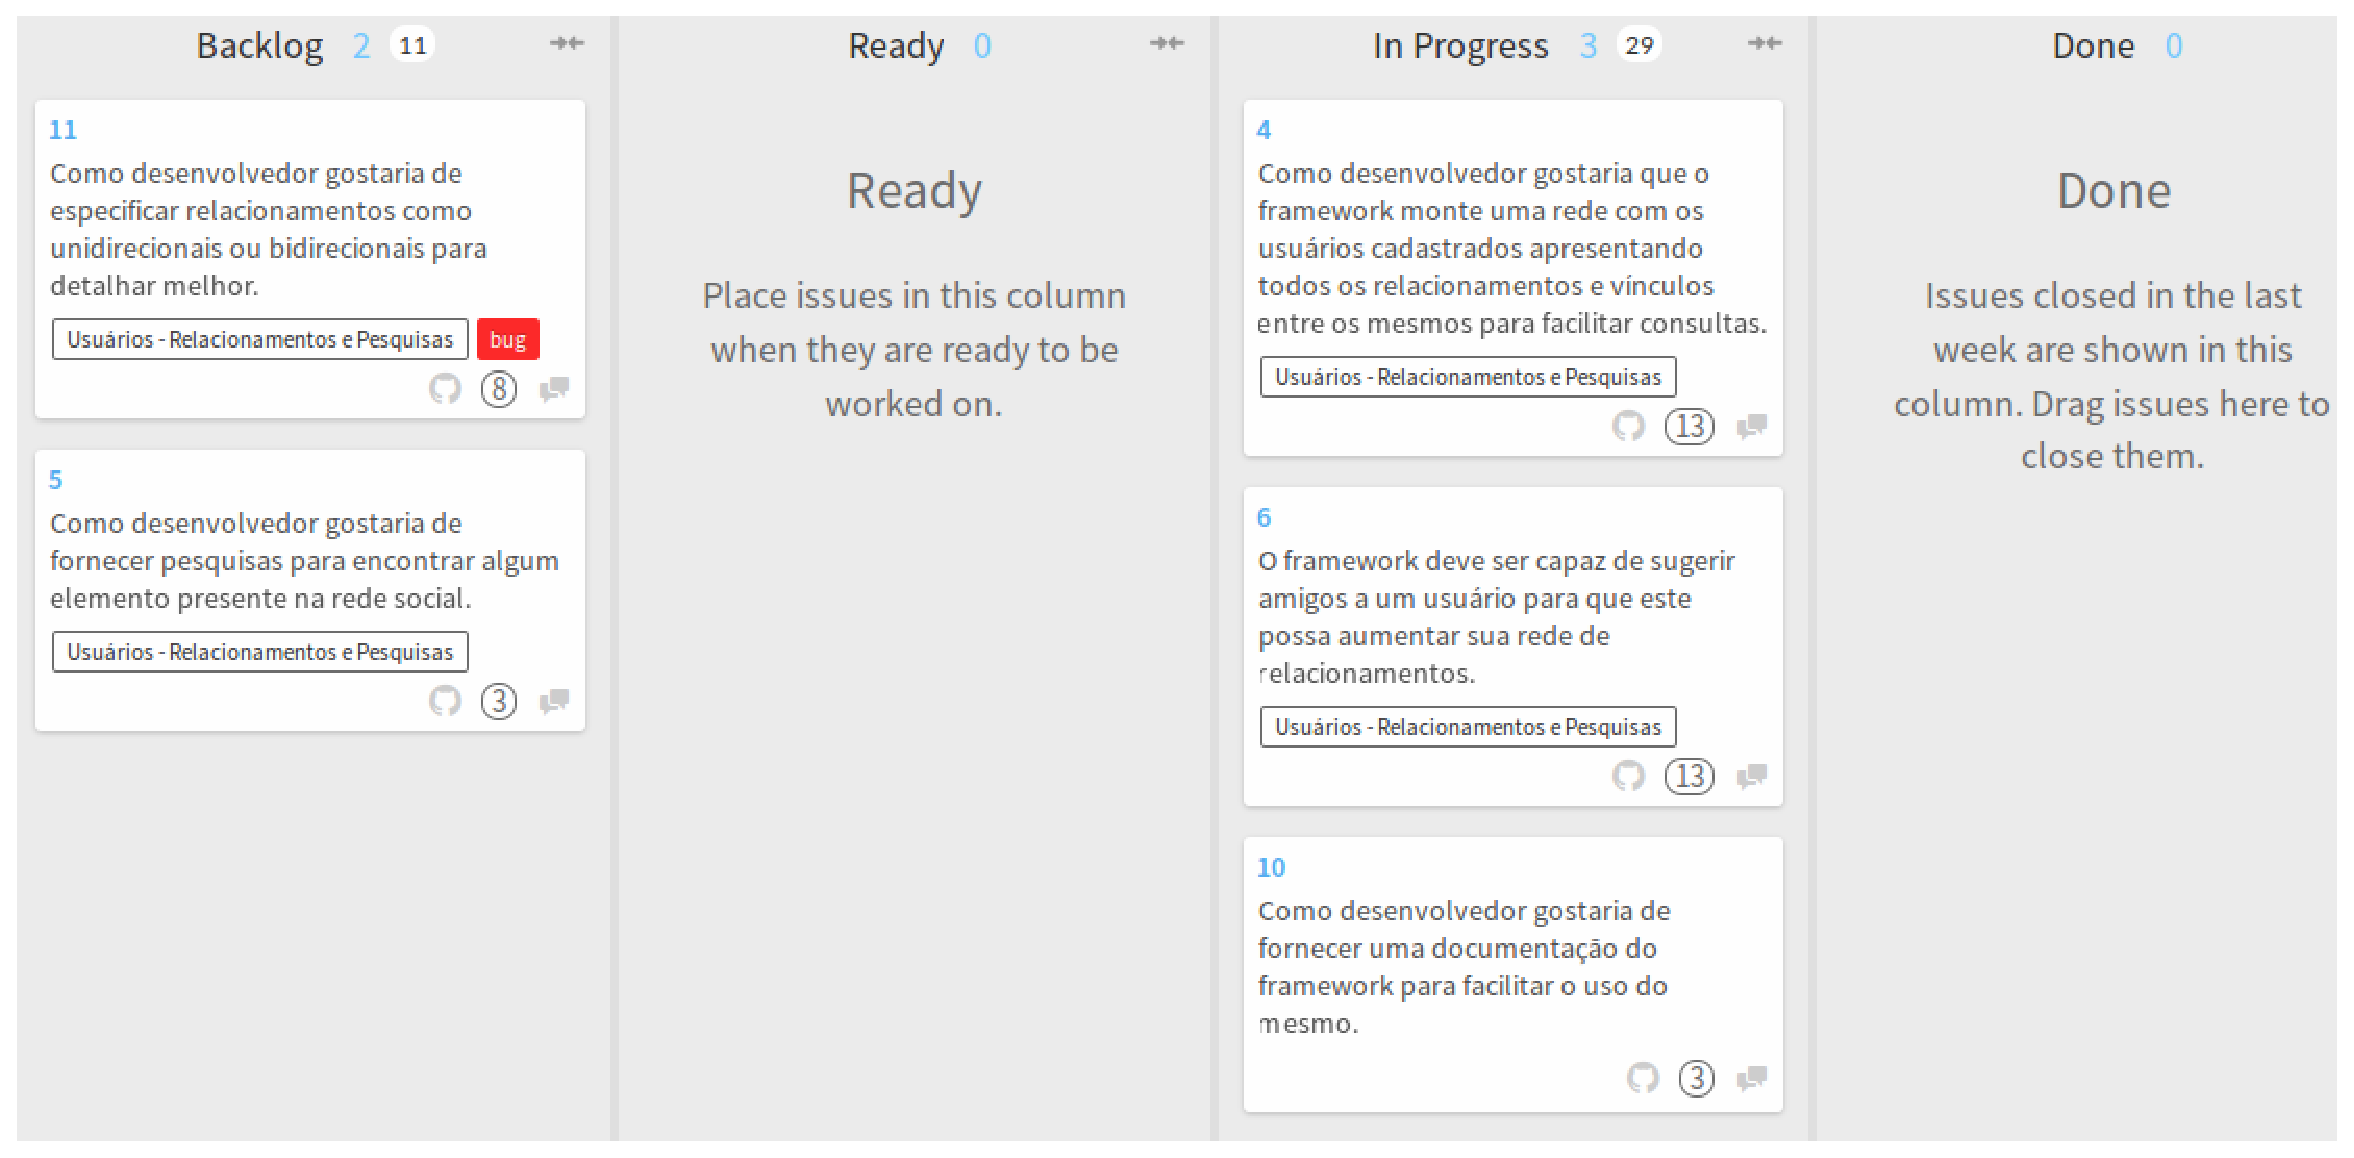
\includegraphics[scale=0.3]{figuras/ferramentas/waffle.eps}
	\caption{Board gerado pelo Waffle}
	\label{waffle}
\end{figure}

\subsection{LaTeX 3}

O \LaTeX\footnote{\url{https://www.latex-project.org}} é um pacote de macros ou marcações para o processador de textos \TeX, utilizado amplamente pela comunidade científica devido à grande qualidade tipográfica. Adicionalmente, torna mais fácil e rápida a produção de documentos em \TeX. O \LaTeX foi desenvolvido por Leslie Lamport a partir do \TeX, criado por Donald Knuth, ambos de código aberto.

O objetivo desse suporte é que o autor se distancie da apresentação visual do trabalho, concentrando-se no seu conteúdo. Para isto, ele possui formas de se lidar facilmente com estruturas como, por exemplo, bibliografias, citações, formatos de páginas e referências. O \LaTeX\ não é algo imutável, e como tal, suporta várias maneiras de estilizar e formatar os documentos.

\subsection{Sublime Text 3}

Este trabalho utilizou o Sublime Text (\textit{build 3103}) como editor de texto. Inicialmente pensado para ser uma extensão do Vim, o Sublime Text\footnote{\url{http://www.sublimetext.com/}} é um editor de texto multiplataforma, escrito em linguagem C++. Com o Sublime é possível automatizar várias tarefas a partir de recursos como, por exemplo, macros, auto-completar, repetição de ações e construção automática.

Outros recursos como dividir a tela em várias janelas, auto \textit{save}, navegação entre páginas por meio de abas e suporte a várias linguagens, por exemplo, C, C++, C\#, CSS, HTML, Java, \LaTeX, PHP, Ruby, SQL, XML, JavaScript e Groovy, fazem do Sublime uma ferramenta popular entre os programadores.

A seguir, na Figura \ref{sublime}, é apresentada uma imagem da ferramenta.

\begin{figure}[!h]
	\centering
	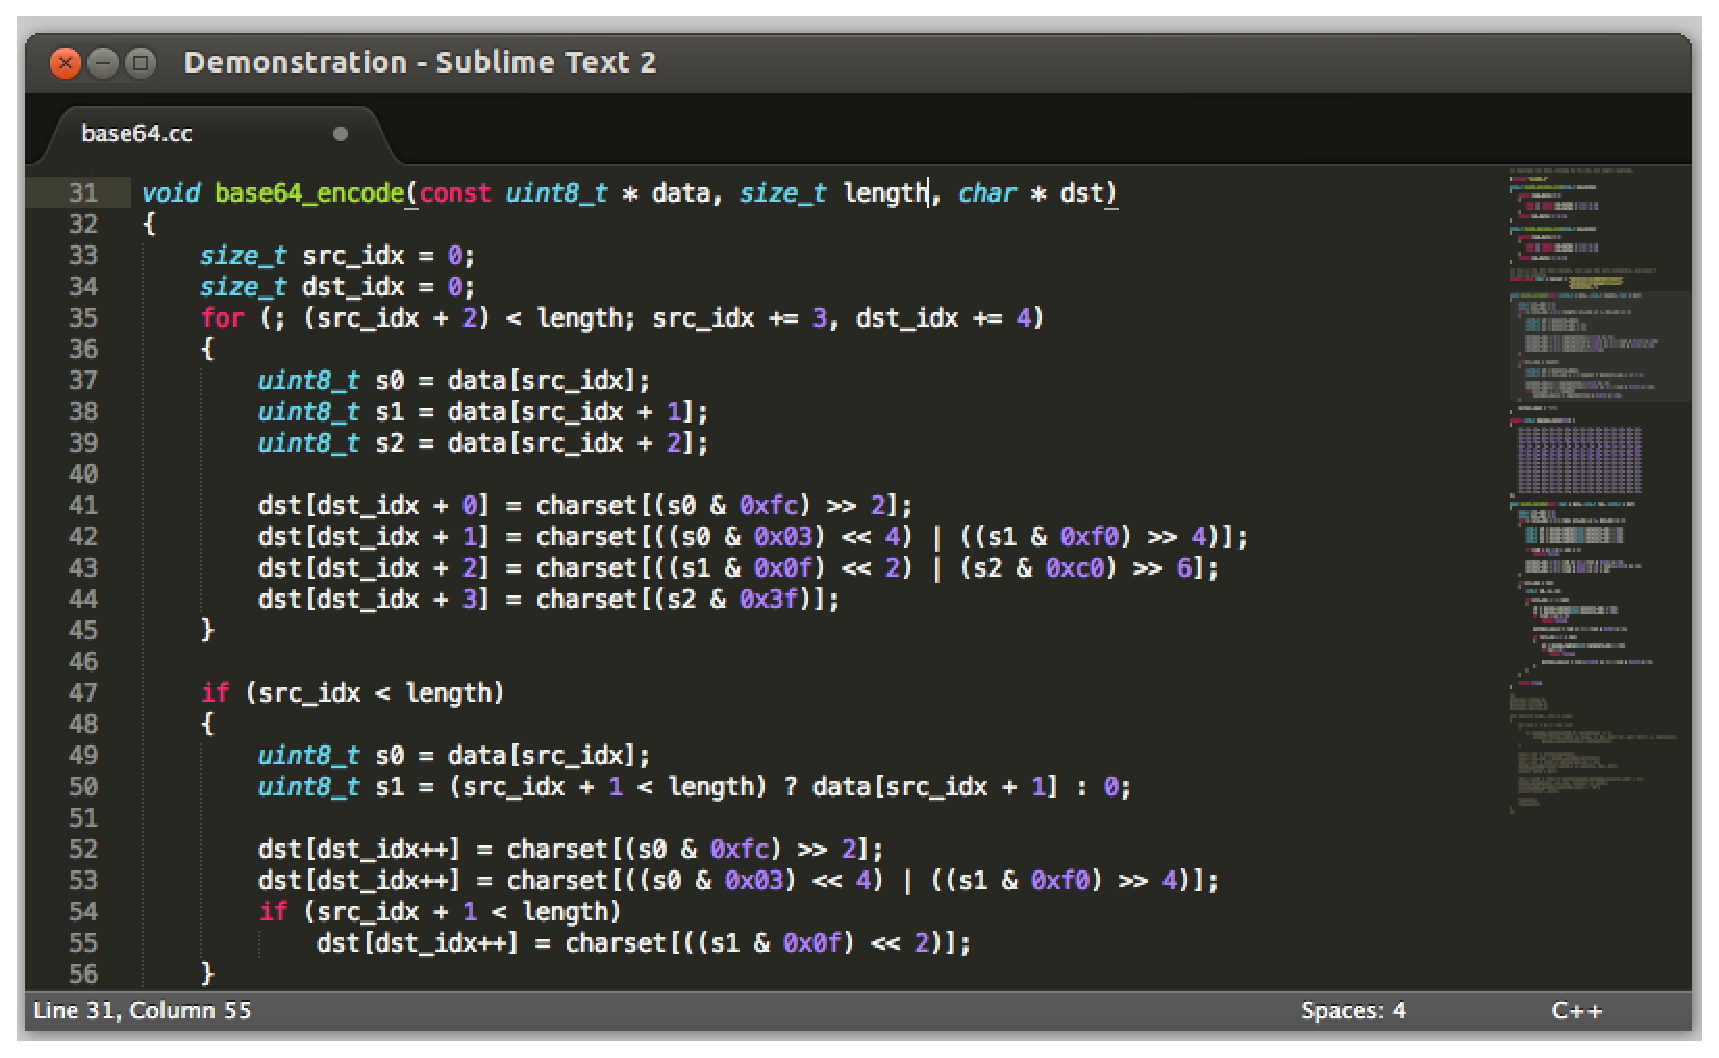
\includegraphics[scale=0.35]{figuras/ferramentas/sublime.eps}
	\caption{Sublime Text 3}
	\label{sublime}
\end{figure}

\subsection{Bizagi Modeler}

Bizagi\footnote{\url{http://www.bizagi.com}} (utilizado na versão 3.0) é uma ferramenta para modelar processos. Esta abrange tanto o mapeamento de processos de trabalho quanto a automação de processos a partir do mapeamento, permitindo que os usuários possam desenhar, documentar e compartilhar seus processos de trabalho usando a notação BPMN (\textit{Business Process Management Notation}). Um diferencial do Bizagi é a possibilidade de realizar tarefas em conjunto, utilizando um ambiente virtual.

A seguir é apresentado um exemplo de uso do Bizagi, na Figura \ref{bizagi}.

\begin{figure}[!h]
	\centering
	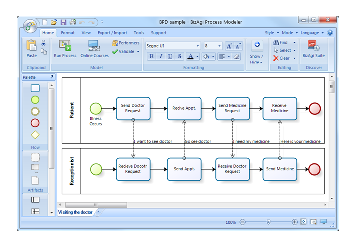
\includegraphics[scale=1.5]{figuras/ferramentas/bizagi.eps}
	\caption{Bizagi Modeler}
	\label{bizagi}
\end{figure}

\subsection{Ubuntu}

Ubuntu\footnote{\url{http://www.ubuntu.com/}} é uma palavra de origem africana que significa: ``Humanidade para os outros'' ou ainda ``Sou o que sou pelo que nós somos''. A distribuição Ubuntu traz o espírito desta palavra para o mundo do software livre. Baseado em Linux e criado a partir do Debian, o Ubuntu é patrocinado pela Canonical Ltda., e é licenciado pela licença GPL (\textit{General License Public}). Para o desenvolvimento deste trabalho foi utilizado o Ubuntu na versão 14.04 LTS.

\subsection{Ruby on Rails}

Ruby on Rails \footnote{\url{http://guides.rubyonrails.org/}} (utilizado na versão 4.2.5) é um \textit{framework} de desenvolvimento de aplicações web escrito na linguagem Ruby, projetado para tornar a programação de aplicações web mais fácil. A filosofia Rails inclui dois princípios orientadores:

\begin{itemize}
	\item \textbf{DRY} (\textit{Don't Repeat Yourself}), ou não repita a si mesmo, é um princípio de desenvolvimento de software que afirma que ``Cada pedaço de conhecimento deve ter uma única representação inequívoca e autoritária dentro de um sistema''\cite{wilson2012practices}.

	\item \textbf{Convenção sobre configuração} é um modelo onde o desenvolvedor precisa definir apenas aspectos não convencionais da aplicação e os aspectos convencionais são pré-estabelecidos. Tal estratégia evita o uso maciço de arquivos de configuração.
\end{itemize}

\end{apendicesenv}
